\documentclass[a4paper,11pt]{article}

\usepackage[spanish]{babel}
\usepackage[utf8]{inputenc}
\usepackage{enumerate}
\usepackage{amsmath}
\usepackage{extsizes}
\usepackage{amssymb}
\usepackage{dsfont}
\usepackage{graphicx}
\usepackage{cancel}
\usepackage[usenames]{color}
\usepackage[dvipsnames]{xcolor}
\usepackage{accents}
\usepackage{flushend}
\usepackage{tikz}
\usepackage[LGR,T1]{fontenc}
\newcommand{\textgreek}[1]{\begingroup\fontencoding{LGR}\selectfont#1\endgroup}
\usetikzlibrary{arrows,automata}
\usepackage{multicol}
\setlength{\columnsep}{1cm}
\usepackage{listings}
\usepackage{graphics,graphicx, float} %para incluir imágenes y colocarlas
\usepackage{caption}
\usepackage{subcaption}



\usepackage[hidelinks]{hyperref}

\usepackage[vmargin=3cm,hmargin=3cm]{geometry}
%\setlength\parindent{0pt}

\setlength\parindent{0pt}


% Carpeta con las imágenes
%\graphicspath{{}}

\begin{document}


	\begin{center}
		\LARGE{\textbf{Nuevos Paradigmas de Interacción (2018-2019)} \\ Grado en Ingeniería Informática \\ Universidad de Granada }
		\vspace*{2.5cm}

		\rule{\textwidth}{1.6pt}\vspace*{-\baselineskip}\vspace*{4pt}
		\rule{\textwidth}{1.6pt}\vspace*{-\baselineskip}\vspace*{2pt}
		\vspace{0.5cm}

		\Huge{Memoria Técnica}

		\vspace{0.5cm}
		\rule{\textwidth}{1.6pt}\vspace*{-\baselineskip}\vspace*{2pt}
		\rule{\textwidth}{1.6pt}\vspace*{-\baselineskip}\vspace*{4pt}

		\vspace{2cm}

\begin{figure}[h!]
	\centering
	
\includegraphics[scale=1]{./Imagenes/logo_informatica.png}
	\label{fig:logougrciencias}
\end{figure}

		\vspace{4cm}
		\LARGE{Ignacio Aguilera Martos, Diego Asterio de Zaballa,\\ Manuel López Roldán \\ 16 de Diciembre de 2018 }

	\end{center}




\newpage

\tableofcontents

\newpage

\section{Idea, dispositivo y plataforma de desarrollo}

El proyecto que hemos querido desarrollar para la tercera práctica con integración de gestos es una continuación de nuestra idea de las dos primeras prácticas. Esta idea era la integración de un museo virtual en realidad aumentada con cuadros, a los que ahora se le suman modelos en 3D tales como esculturas o edificios que son manejados mediante gestos leídos con el dispositivo Leap Motion.

\vspace{10px}

El dispositivo escogido ha sido Leap Motion ya que es un dispositivo cuyo último SDK está pensado y desarrollado para la integración con las gafas de realidad virtual con lo que la integración con nuestra aplicación sería muy coherente. El dispositivo iría pegado a las gafas de tal forma que el usuario puede realizar los gestos sin necesidad de colocarse en un punto concreto o encima de algún elemento concreto puesto que los gestos son leídos directamente desde el Leap que apunta siempre a las manos por su localización en las gafas de VR. En este sentido la aplicación aún no está preparada para poder comunicarse con el dispositivo móvil puesto que es el componente que falta por desarrollar por el equipo de Leap Motion Inc. y que ya han anunciado que están trabajando en esta integración. De momento el Leap puede emplearse como lo hemos integrado nosotros, es decir desde el ordenador, con el cuál si tiene una integración gestual sólida.

\vspace{10px}

Cabe decir que la plataforma que hemos elegido para el desarrollo de la aplicación ha sido Unity 3D. Esta decisión viene motivada por la facilidad de uso que nos da este entorno de desarrollo en el ámbito tridimensional así como la fácil integración de Leap Motion y reconocimiento de los datos provistos por el dispositivo ya que sus desarrolladores han implementado un Asset de Unity para facilitar el manejo del mismo. La integración por tanto con nuestra anterior idea del museo sería muy sencilla puesto que ambos proyectos están implementados en Unity y por tanto sólo se necesitaría diferenciarlos en dos escenas que serían cargadas convenientemente en función de si se quieren visualizar los cuadros o los modelos 3D.

\vspace{10px}

Una vez explicado esto, para desarrollar mejor la idea del proyecto, vamos a dar una introducción más específica sobre lo implementado para luego desgranar los aspectos técnicos del mismo.

\section{Proyecto}

El proyecto nos muestra nuestras manos reconocidas por el Leap Motion para poder interactuar adecuadamente con los objetos y poder ver cuándo los estamos tocando. La primera pantalla que se nos muestra es un menú tridimensional que es accedido presionando las opciones tal y como se muestra en los proyectos de ejemplo del Leap Motion. El menú nos da las cuatro opciones que tenemos para poder navegar e interactuar con las esculturas del museo que son: Observation Mode, Free World Mode, Play Mode y Exit.
\begin{itemize}
	\item Observation Mode: El Observation Mode nos permite visualizar la estatua en 3D como un modelo que se presenta en el centro de la escena y con la cual podemos interactuar gestualmente para desplazarla como queramos o hacerle zoom.
	\item Free World Mode: Este modo es el que nos permitirá visualizar la escena con realidad aumentada una vez que el SDK de Leap Motion tenga disponible la comunicación entre el dispositivo y el propio smartphone.
	\item Play Mode: Con este modo tenemos disponible un mundo con físicas que nos permite interactuar con elementos como cubos o la propia estatua para poder jugar desplazando los elementos, manipulándolos o tirándolos.
	\item Exit: Nos permite salir de la aplicación.
\end{itemize}

A continuación vamos a detallar más la estructura general de la escena para poder entrar posteriormente más en profundidad en cada modo y los gestos desarrollados.

\section{Estructura de la escena}

Para comenzar vamos a visualizar un esquema de los nodos principales de la escena:

\begin{figure}[!h]
	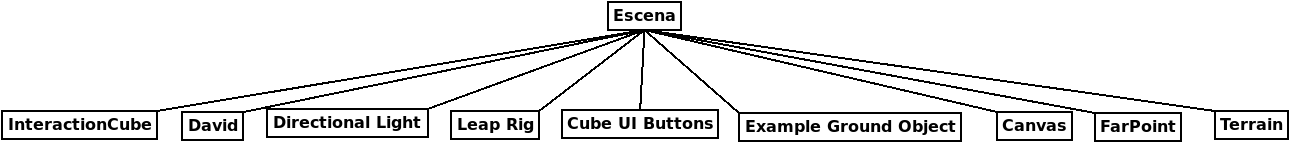
\includegraphics[scale=0.5]{./Imagenes/Escena.png}
	\caption{Diagrama de la escena principal}
	\label{escena}
\end{figure}

Como podemos observar la escena contiene 8 elementos en total que vamos a explicar a continuación:

\begin{itemize}
	\item InteractionCube, FarPoint, Terrain y David: estos elementos son los que componen el modelo tridimensional del David de Miguel Ángel (estatua que se muestra en nuestra aplicación). Este conjunto hace que tengamos una `hitbox' con la que interactuar con el modelo así como un terreno para prevenir de que desaparezca de la escena. Este último elemento es empleado cuando activamos el Play Mode ya que las figuras de la escena ganan propiedades de físicas con lo que podemos interactuar con ellos y para lo que necesitamos un plano inferior que nos haga de suelo para que la gravedad no se lleve los elementos hacia abajo indefinidamente.
	\item Directional Light: este elemento de la escena nos da la forma en la que la luz se aplica sobre la escena. Es el objeto que provee de una fuente de luz a la misma.
	\item Leap Rig: este elemento de la escena es el que contiene la funcionalidad y las características del Leap Motion así como la recopilación de los datos del mismo para que posteriormente se puedan utilizar en nuestro script de detección de gestos. Viene incorporado en el Asset provisto por los desarrolladores de Leap Motion Inc. para Unity.
	\item Cube UI Buttons: este elemento incorpora los botones con los que se puede interactuar mediante las manos virtuales de las que nos provee el SDK de Leap Motion.
	\item Canvas: en este nodo del gafo de la escena tenemos los textos que se incorporan en los botones para poder distinguirlos entre sí de forma visual.
\end{itemize}

No sólo tenemos estos elementos dentro de la escena, si no que también hay algunos nodos que contienen subnodos relevantes en el desarrollo del proyecto y de los cuales haremos una breve explicación para exponer su utilidad dentro del mismo.

\vspace{10px}

En primer lugar explicaremos el árbol que obtenemos del nodo Leap Rig:

\begin{figure}[!h]
	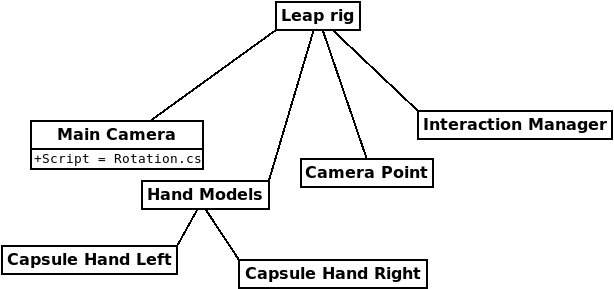
\includegraphics[scale=0.5]{./Imagenes/Leap_Rig.png}
	\caption{Diagrama del nodo Leap Rig}
	\label{leapRig}
\end{figure}

\begin{itemize}
	\item Main Camera y Camera Point: estos elementos representan la cámara de la escena, esto es, dónde estará por defecto el usuario, permitiendo además cambiar el foco de atención a diferentes zonas de la misma si lo requiere. Sobre estos elementos de la escena es sobre los que se coloca el script Rotation.cs que es el que contiene el código referente a los gestos implementados y que posteriormente explicaremos.
	\item Hand Models: Estos elementos son los que implementan el modelo tridimensional de las manos que interactúa y se mueve con respecto a las nuestras mediante el dispositivo Leap Motion. Gracias a estos modelos la experiencia del usuario es mucho más fácil ya que así tiene una percepción real de dónde están sus manos virtuales en la escena.
	\item Interaction Manager: Este componente contiene el procesamiento de la información de las manos mediante el Leap e integra la compatibilidad con VR para Oculus y HTC Vive. Dentro de este objeto tenemos un interactuador para cada mano que recoge la información sobre cada dedo (si está o no extendido), sobre la velocidad de cada mano y sobre el vector de dirección y el vector normal de la palma de la mano. Esta información será accedida posteriormente para la elaboración de los gestos.
\end{itemize}

\vspace{20px}

También tenemos elementos en el nodo Cube UI Buttons los cuales son los propios botones para cada opción.

\begin{figure}[!h]
	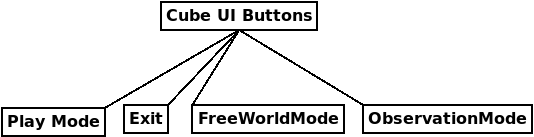
\includegraphics[scale=0.57]{./Imagenes/Cube_UI_Buttons.png}
	\caption{Diagrama de Cube UI Buttons}
	\label{cubeUIButtons}
\end{figure}

Cada uno de estos botones contiene un objeto de tipo Button Cube que son los botones con los que Leap puede interactuar presionándolos y que vienen incluidos en el Asset de Leap Motion.

\vspace{10px}

Asimismo tenemos que del nodo Canvas cuelgan los textos que se superponen sobre los botones.

\begin{figure}[!h]
	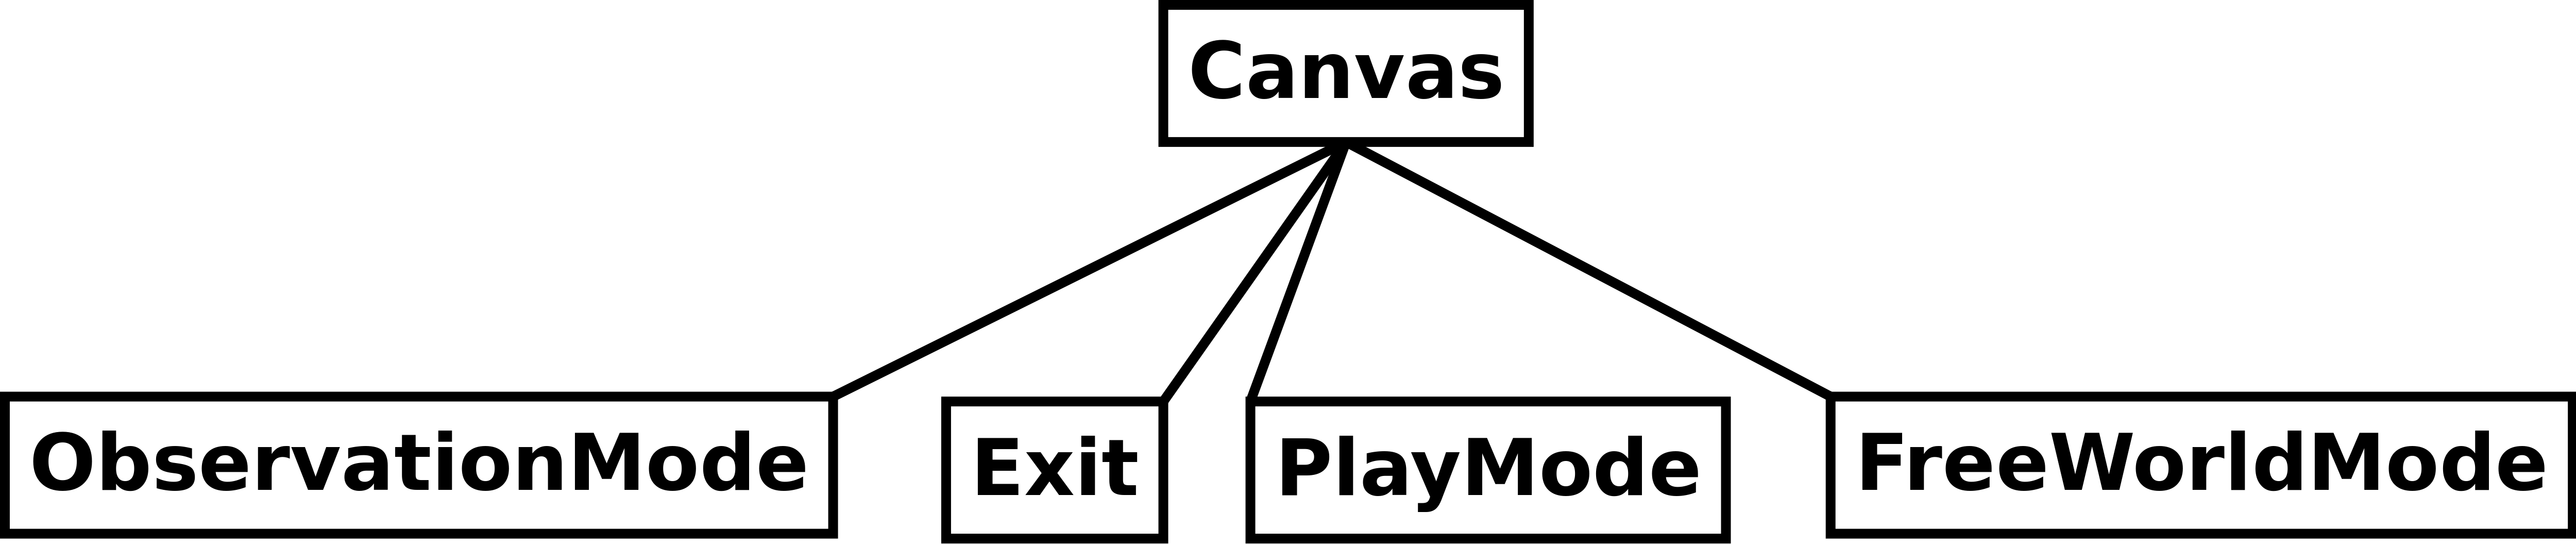
\includegraphics[scale=0.56]{./Imagenes/Canvas.png}
	\caption{Diagrama del nodo Canvas}
	\label{canvas}
\end{figure}

Estos textos se enlazan al botón correspondiente del nodo Cube UI Buttons.

\section{Gestos}

Para poder realizar la implementación de los gestos primero tenemos que comprender qué información obtenemos del dispositivo Leap Motion y cómo se almacena la misma. 

\vspace{10px}

Para debemos inicializar un elemento de tipo Controller del que obtendremos un objeto de tipo Frame llamando al método `\textbf{Frame()}'. Este objeto es el que contiene toda la información que el dispositivo recopila de las manos.

\vspace{10px}

Las manos se guardan en un elemento de tipo `\textbf{List<Hands>}' por orden de detección del dispositivo, esto es, no tenemos la certeza de que la primera mano que tenemos en el vector de manos sea la izquierda o la derecha. Para consultar esta información tenemos el método `\textbf{hand.IsRight()}' o `\textbf{hand.IsLeft()}' los cuales nos dan la información sobre qué mano es la que tenemos en escena. Además podemos obtener más información de la mano pero nosotros sólo hemos empleado dos datos más. El primero de ellos es la velocidad de movimiento de la palma de la mano que es obtenida accediendo al atributo `\textbf{hand.PalmVelocity}'. Con esto podemos saber si nos estamos moviendo más o menos rápido. Además podemos obtener la dirección en la que estamos moviendo la mano con el último dato que hemos necesitado en nuestro proyecto que es el vector normal a la palma de la mano. Este dato lo obtenemos mediante el atributo `\textbf{hand.PalmNormal}'.

\vspace{10px}

Además de la información genérica sobre la mano tenemos un vector con cada dedo detectado por el Leap Motion. Para acceder a esta lista de dedos lo haremos mediante el atributo `\textbf{hand.Fingers}' en la cual tendremos 5 posiciones, una para cada dedo. De cada uno de estos dedos hemos obtenido dos tipos de datos. El primero de ellos es información sobre si está o no extendido. Para poder obtener dicho dato lo debemos hacer accediendo al atributo `\textbf{finger.IsExtended}' que nos devolverá verdadero si el dedo está extendido y falso si no lo está. Además hemos obtenido la posición de cada dedo como vector tridimensional. Para acceder a dicho dato lo hacemos mediante el atributo `\textbf{finger.TipPosition}'.

\vspace{10px}

Tras haber comentado cómo hemos obtenido cada dato sobre la mano y los dedos pasamos a realizar una explicación de los gestos implementados.

\subsection{Traer la estatua a primer plano}

Lo primero que tenemos que hacer es traer la estatua a primer plano de la escena ya que por defecto al entrar en el modo Observation Mode veremos que nos aparece muy alejada de nosotros y no podemos interactuar con ella adecuadamente. Para acercarla tendremos que realizar un gesto que consiste en tener la mano derecha extendida y contraer los dedos de la siguiente forma:

\begin{figure}[!h]
	\centering
	\begin{subfigure}{0.48\textwidth}
		\centering
		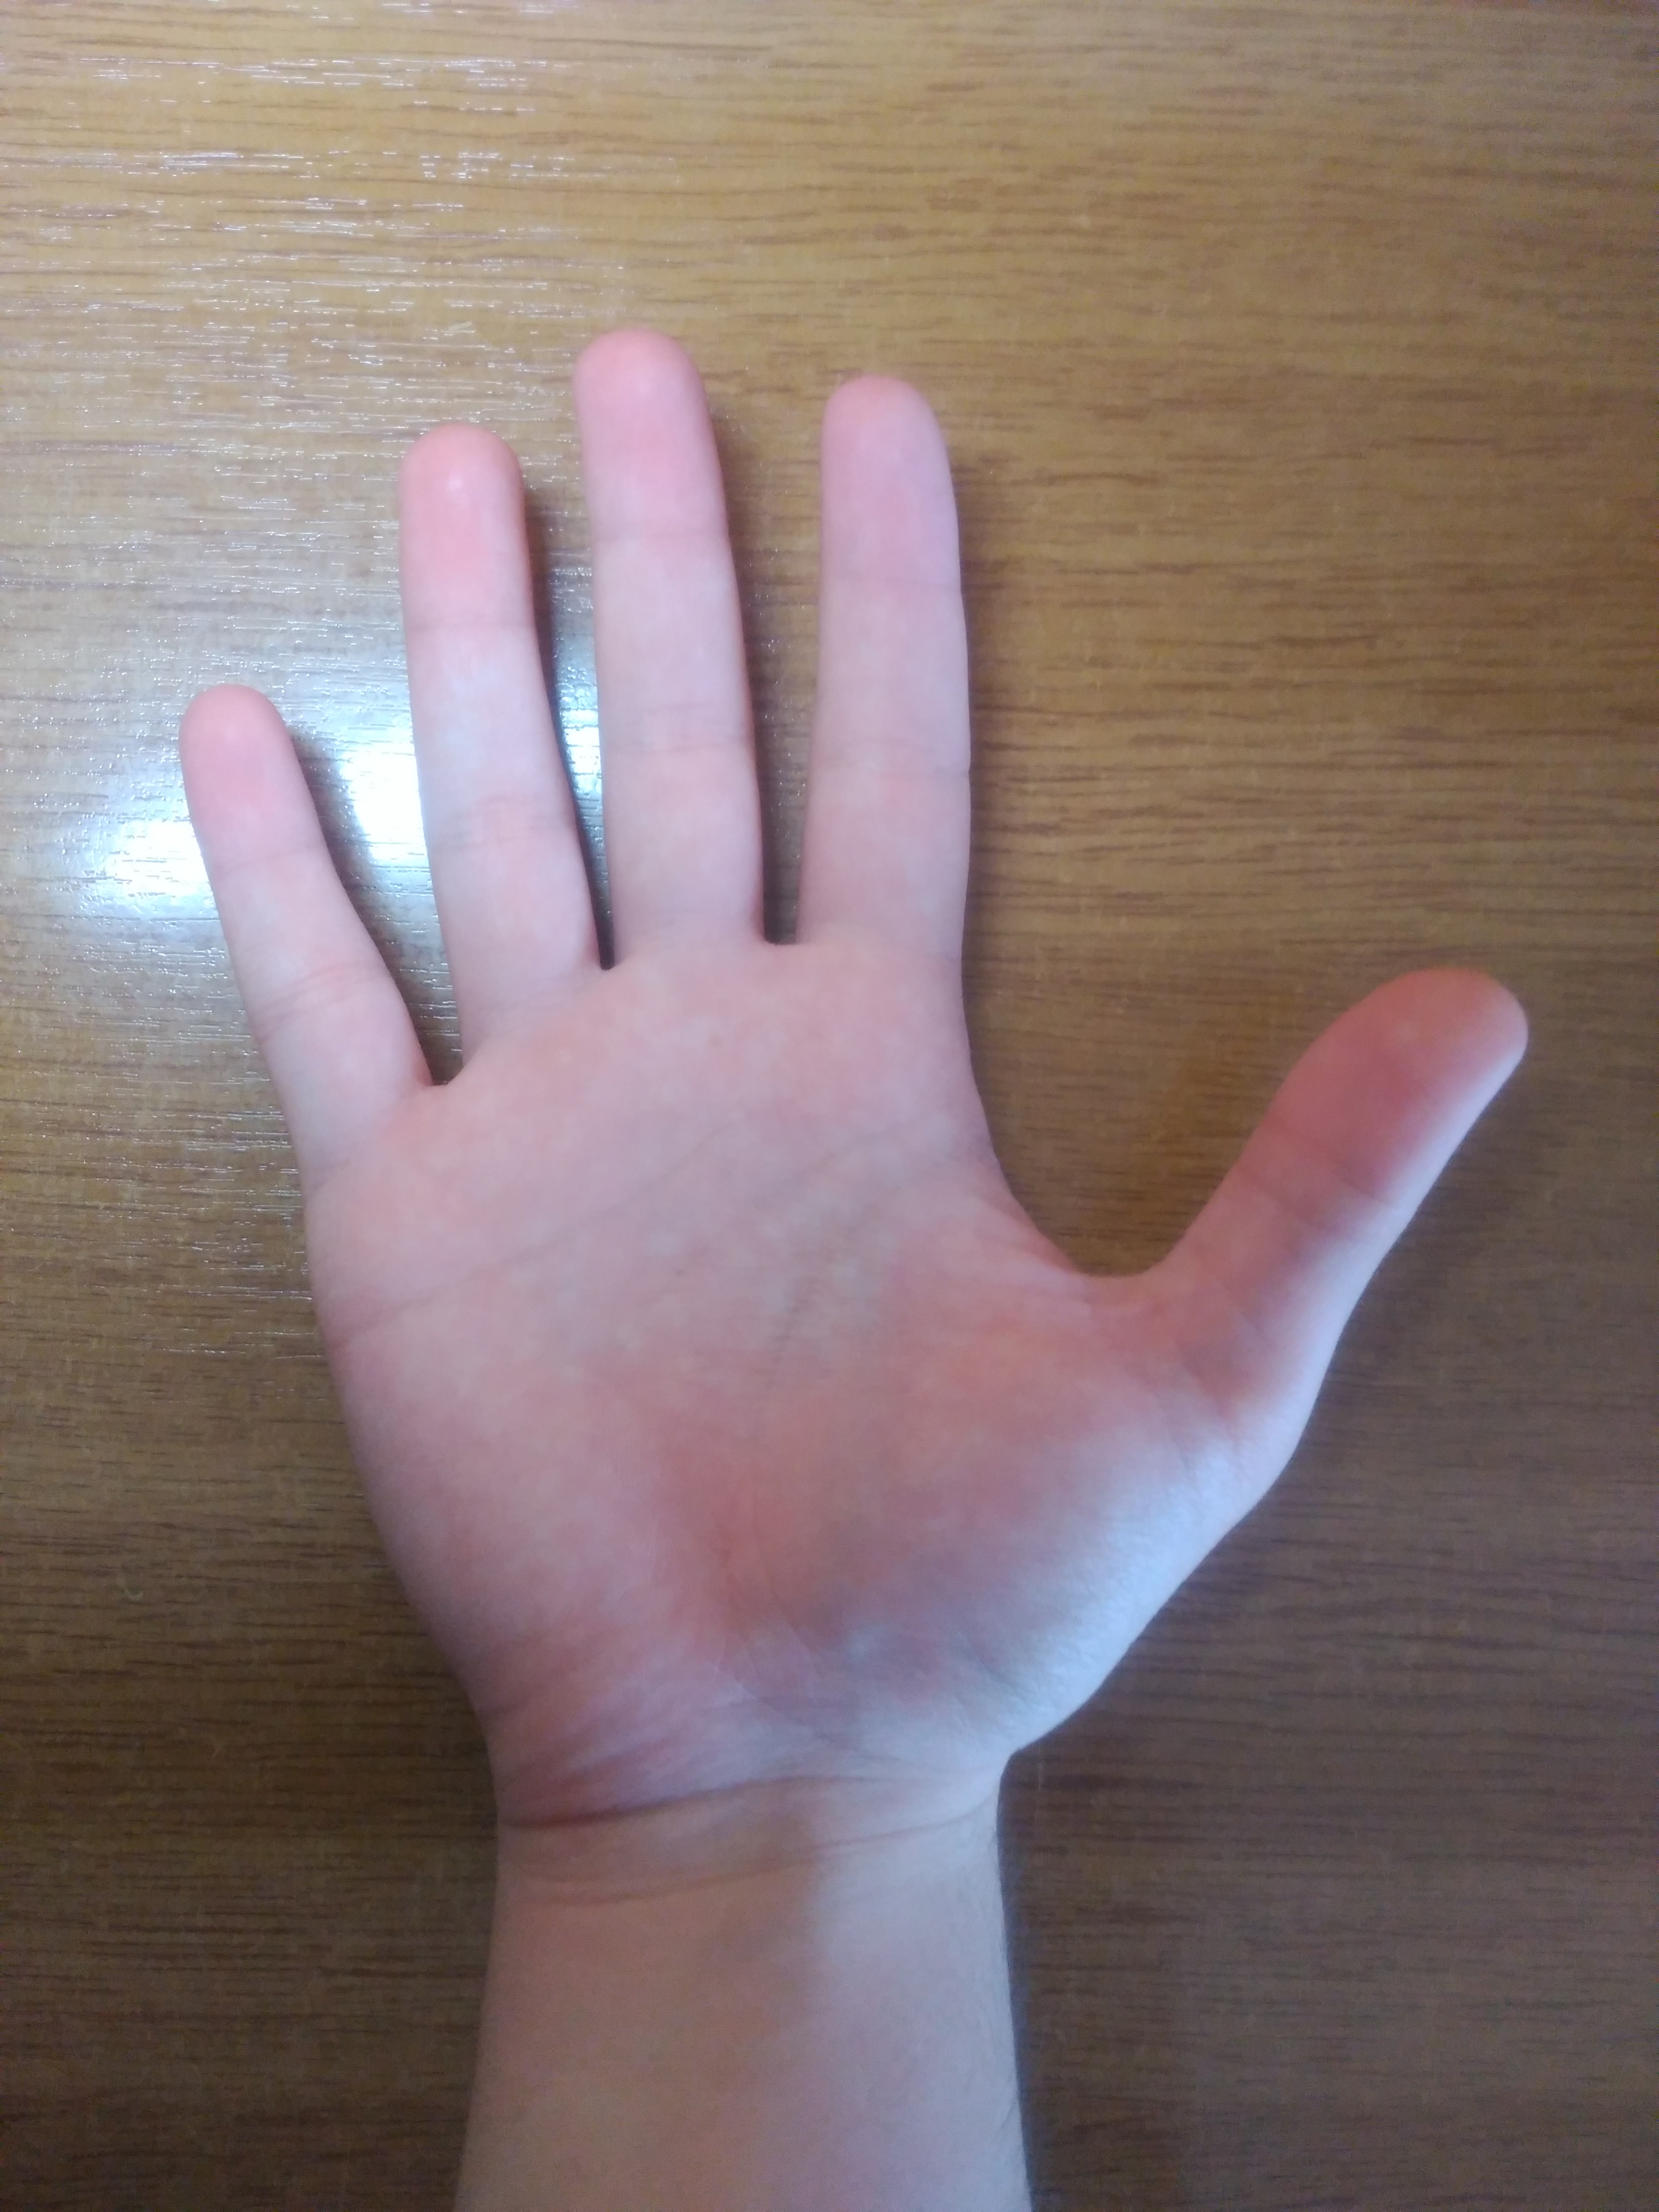
\includegraphics[scale=0.066]{./Imagenes/trae_da_vinci1.jpg}
		\caption{Mano derecha extendida}
	\end{subfigure}
	\begin{subfigure}{0.48\textwidth}
		\centering
		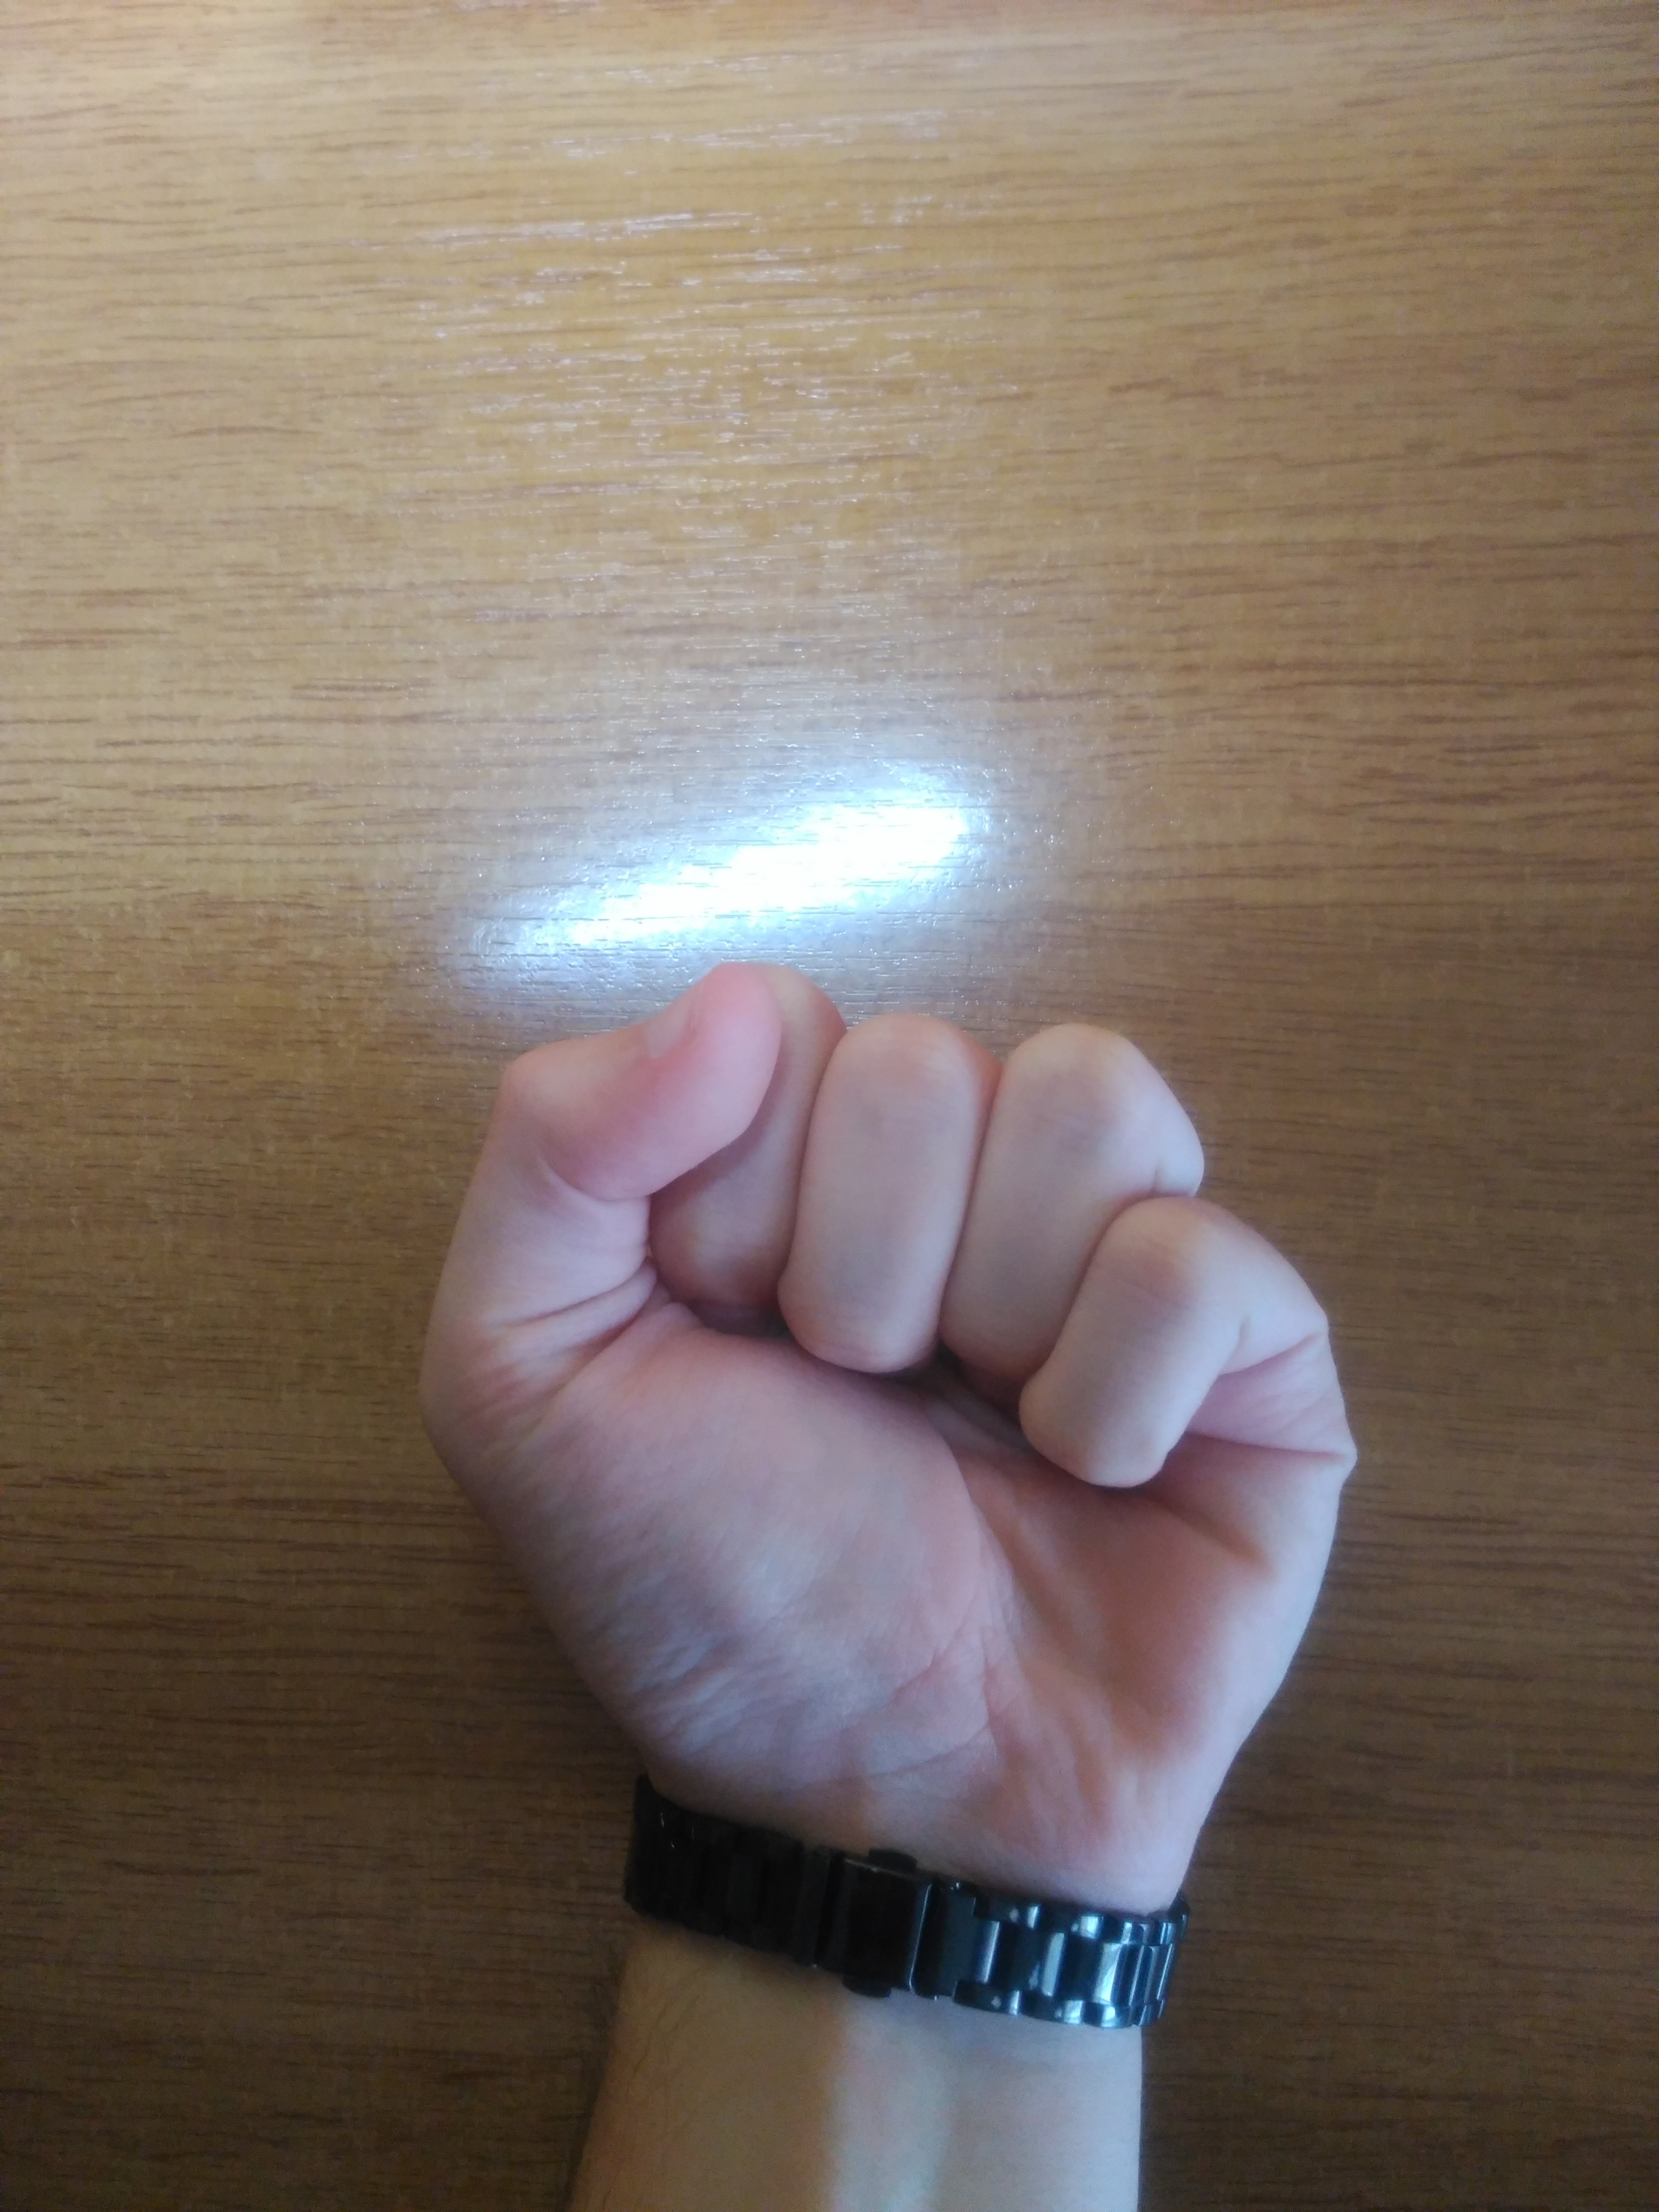
\includegraphics[scale=0.066]{./Imagenes/trae_da_vinci2.jpg}
		\caption{Mano derecha contraída}
	\end{subfigure}
	\caption{Gesto para traer la figura a primer plano}
	\label{gesto1}
\end{figure}

Este gesto requiere controlar si todos los dedos estaban o no contraídos en el instante anterior. Para esto hemos controlado el evento mediante un booleano que se actualiza en cada instante mediante la función `\textbf{Update()}'. Para ello comprobamos si los dedos están extendidos mediante el atributo anteriormente mencionado y actualizamos el valor en el último momento del método `\textbf{Update()}'. Antes de esta actualización comprobamos si los dedos estaban en el instante anterior extendidos o contraídos y su estado actual con lo que podemos saber si estamos abriendo y cerrando la mano y por tanto haciendo el gesto.

\vspace{10px}

Cabe decir además que este gesto es únicamente hecho con la mano derecha, por lo que debemos controlar también que la única mano que es detectada por el Leap Motion sea la que nosotros queremos mediante el atributo `\textbf{hand.IsRight}'.

\subsection{Rotación con respecto al eje Y}

Esta acción involucra dos gestos opuestos para poder realizar la acción. El objetivo de este gesto es que la estatua gire en sentido horario o antihorario entorno al eje Y para poder ver todos los perfiles de la misma. El gesto consiste en inclinar la mano hacia un lado u otro para girar la estatua en un sentido o el opuesto. Veamoslo en una imagen:

\begin{figure}[!h]
	\centering
	\begin{subfigure}{0.32\textwidth}
		\centering
		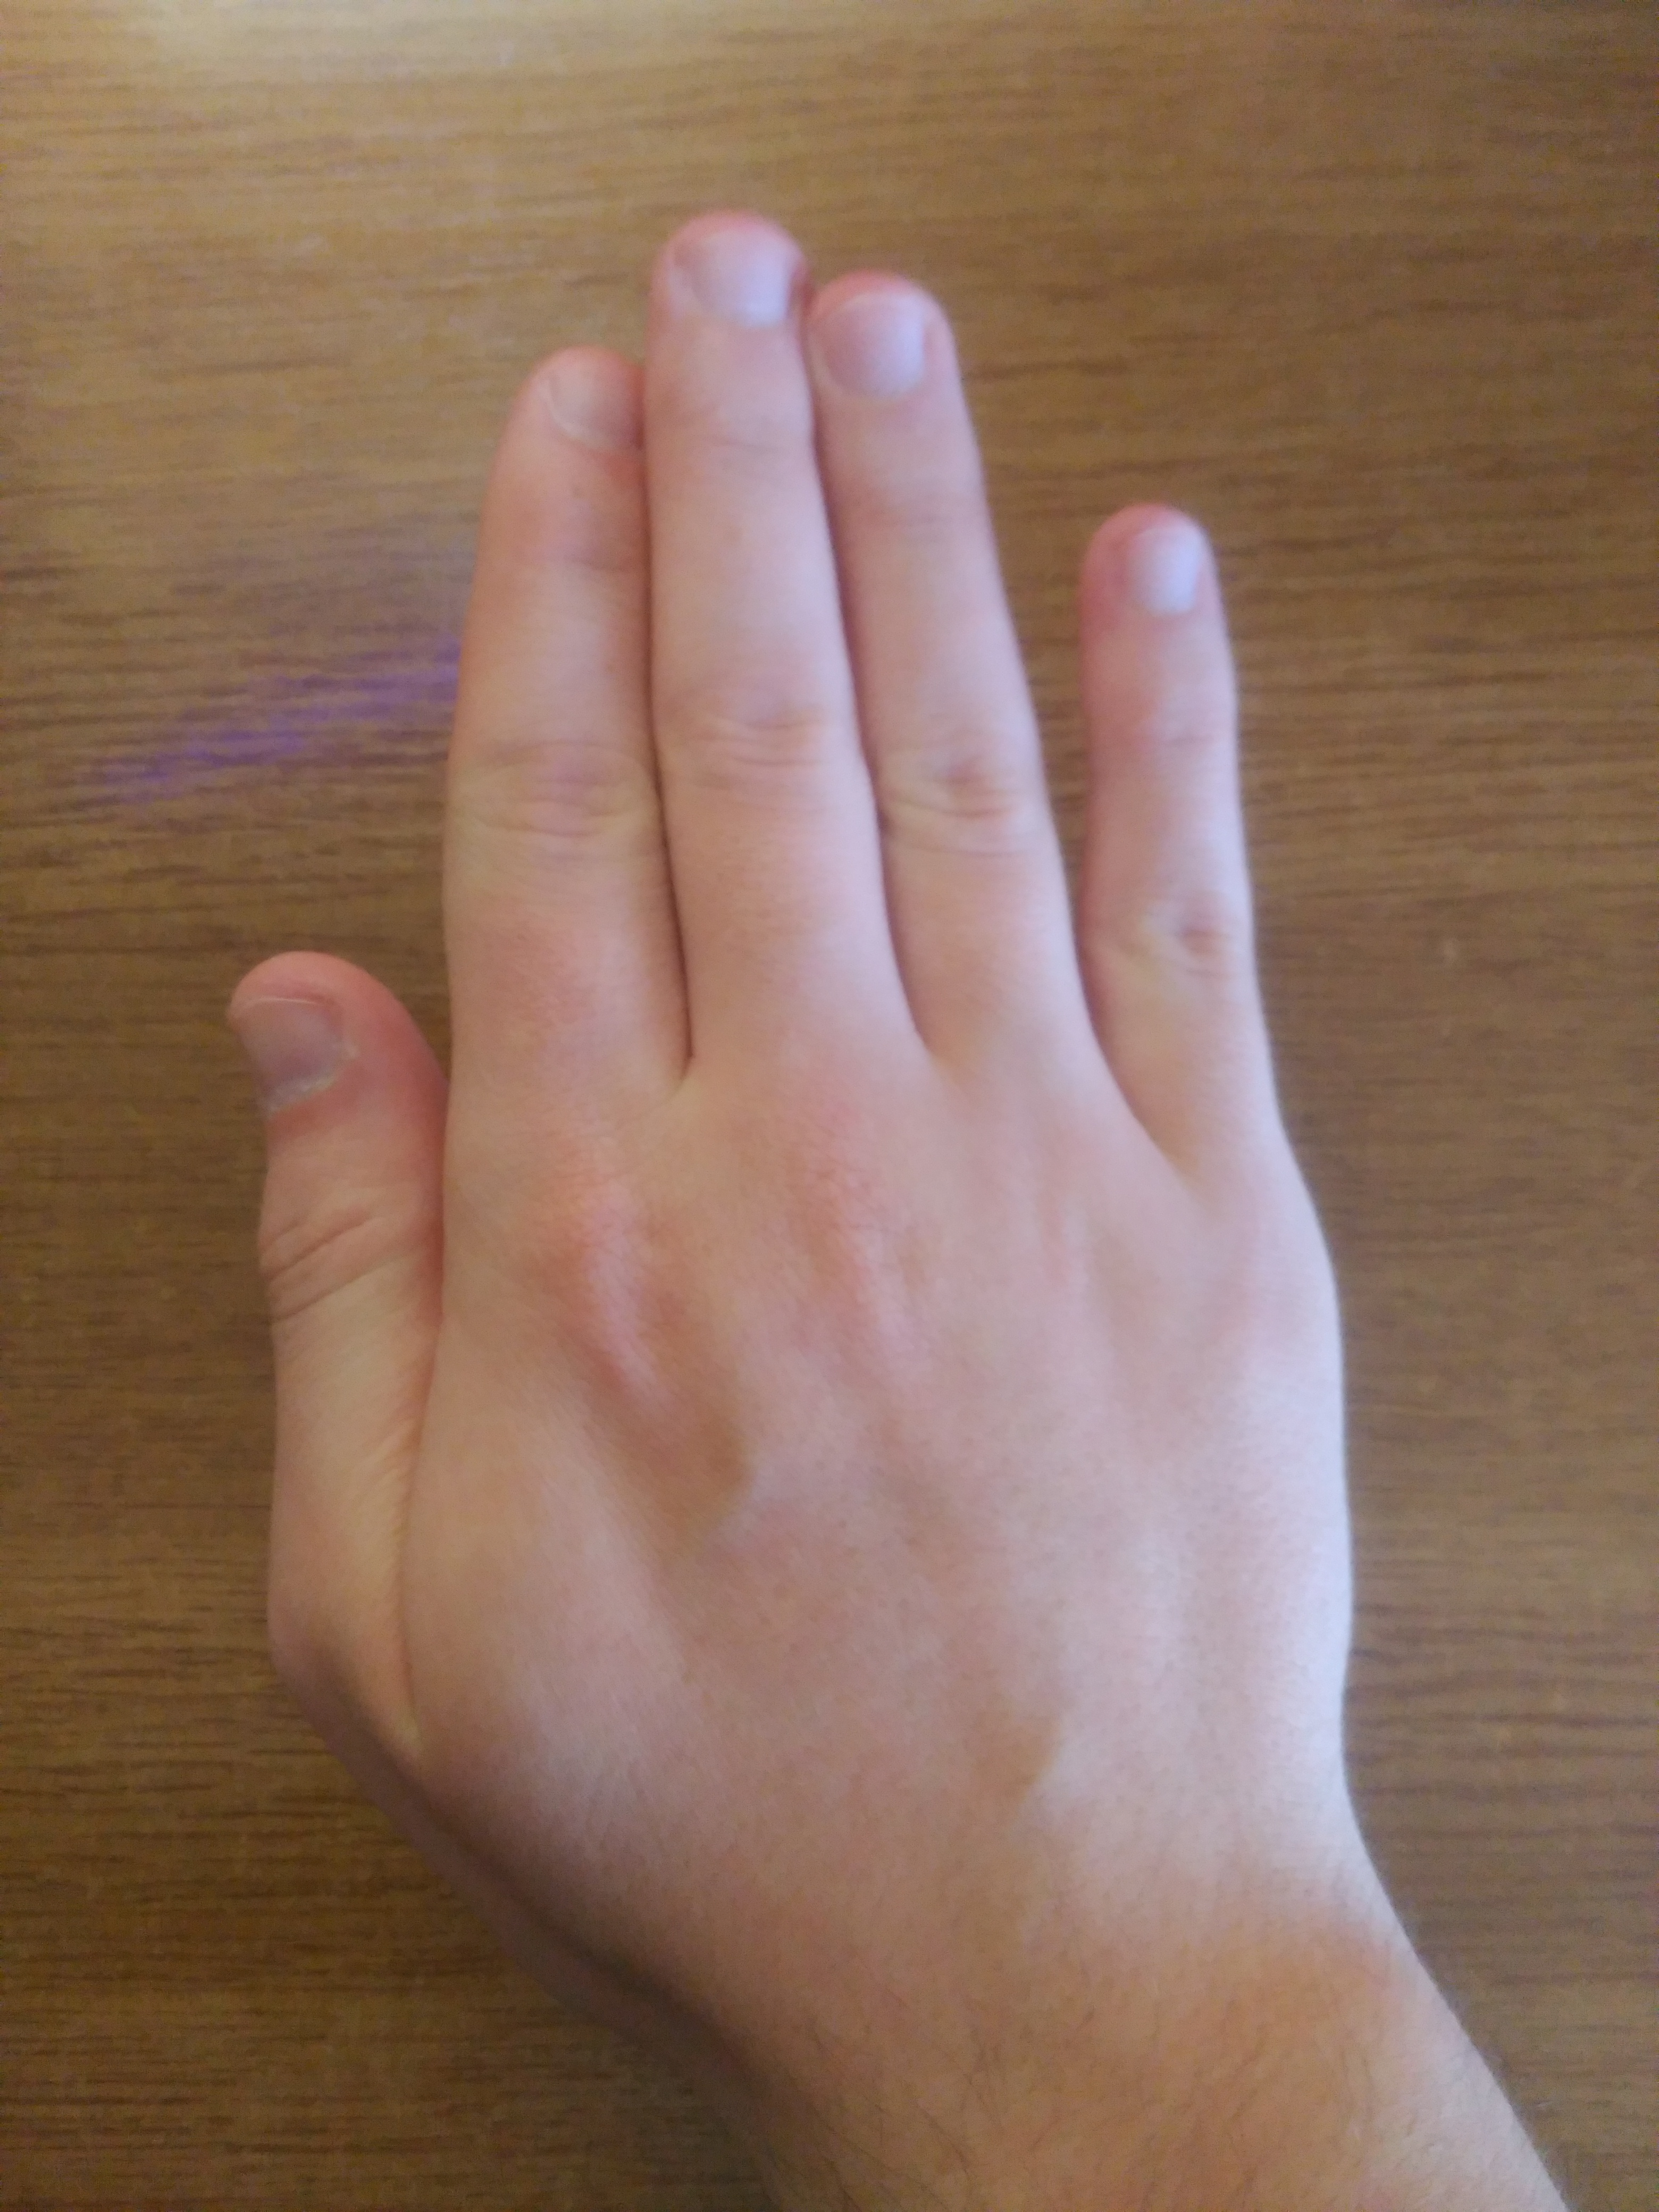
\includegraphics[scale=0.044]{./Imagenes/normal.jpg}
		\caption{Mano sin inclinar}
	\end{subfigure}
	\begin{subfigure}{0.33\textwidth}
		\centering
		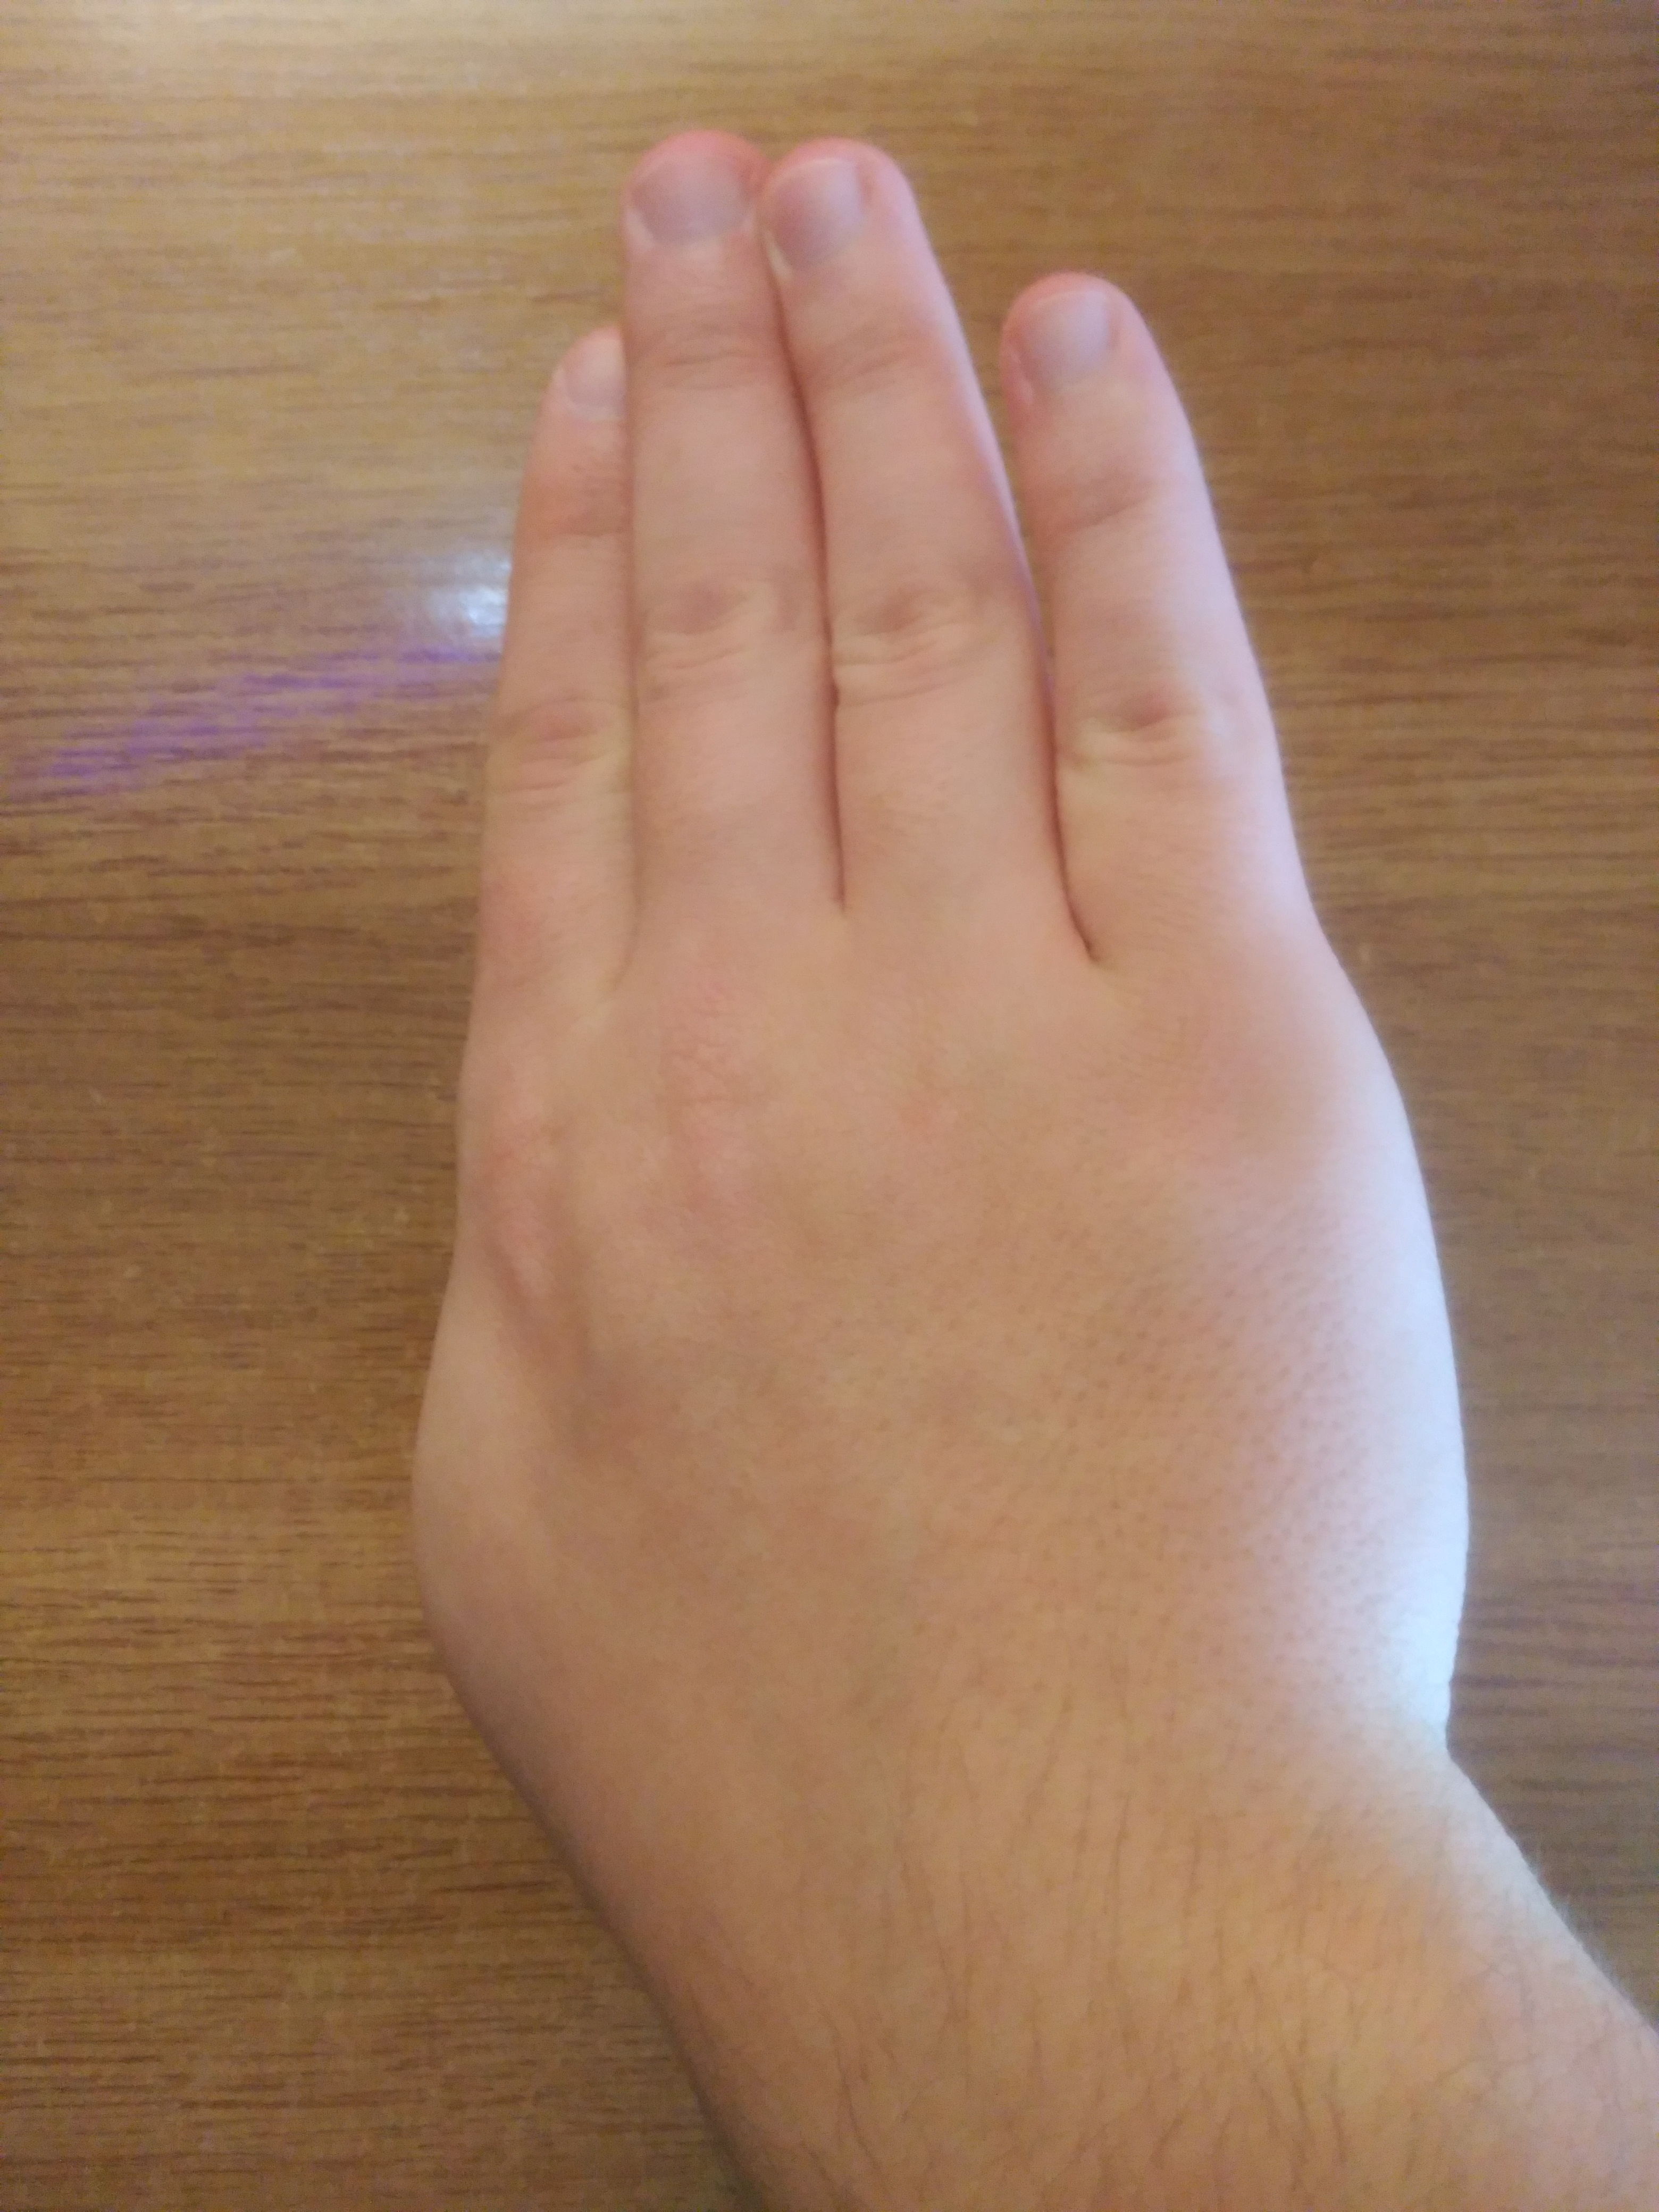
\includegraphics[scale=0.044]{./Imagenes/rota_horario.jpg}
		\caption{Mano hacia a la izquierda}
	\end{subfigure}
	\begin{subfigure}{0.33\textwidth}
		\centering
		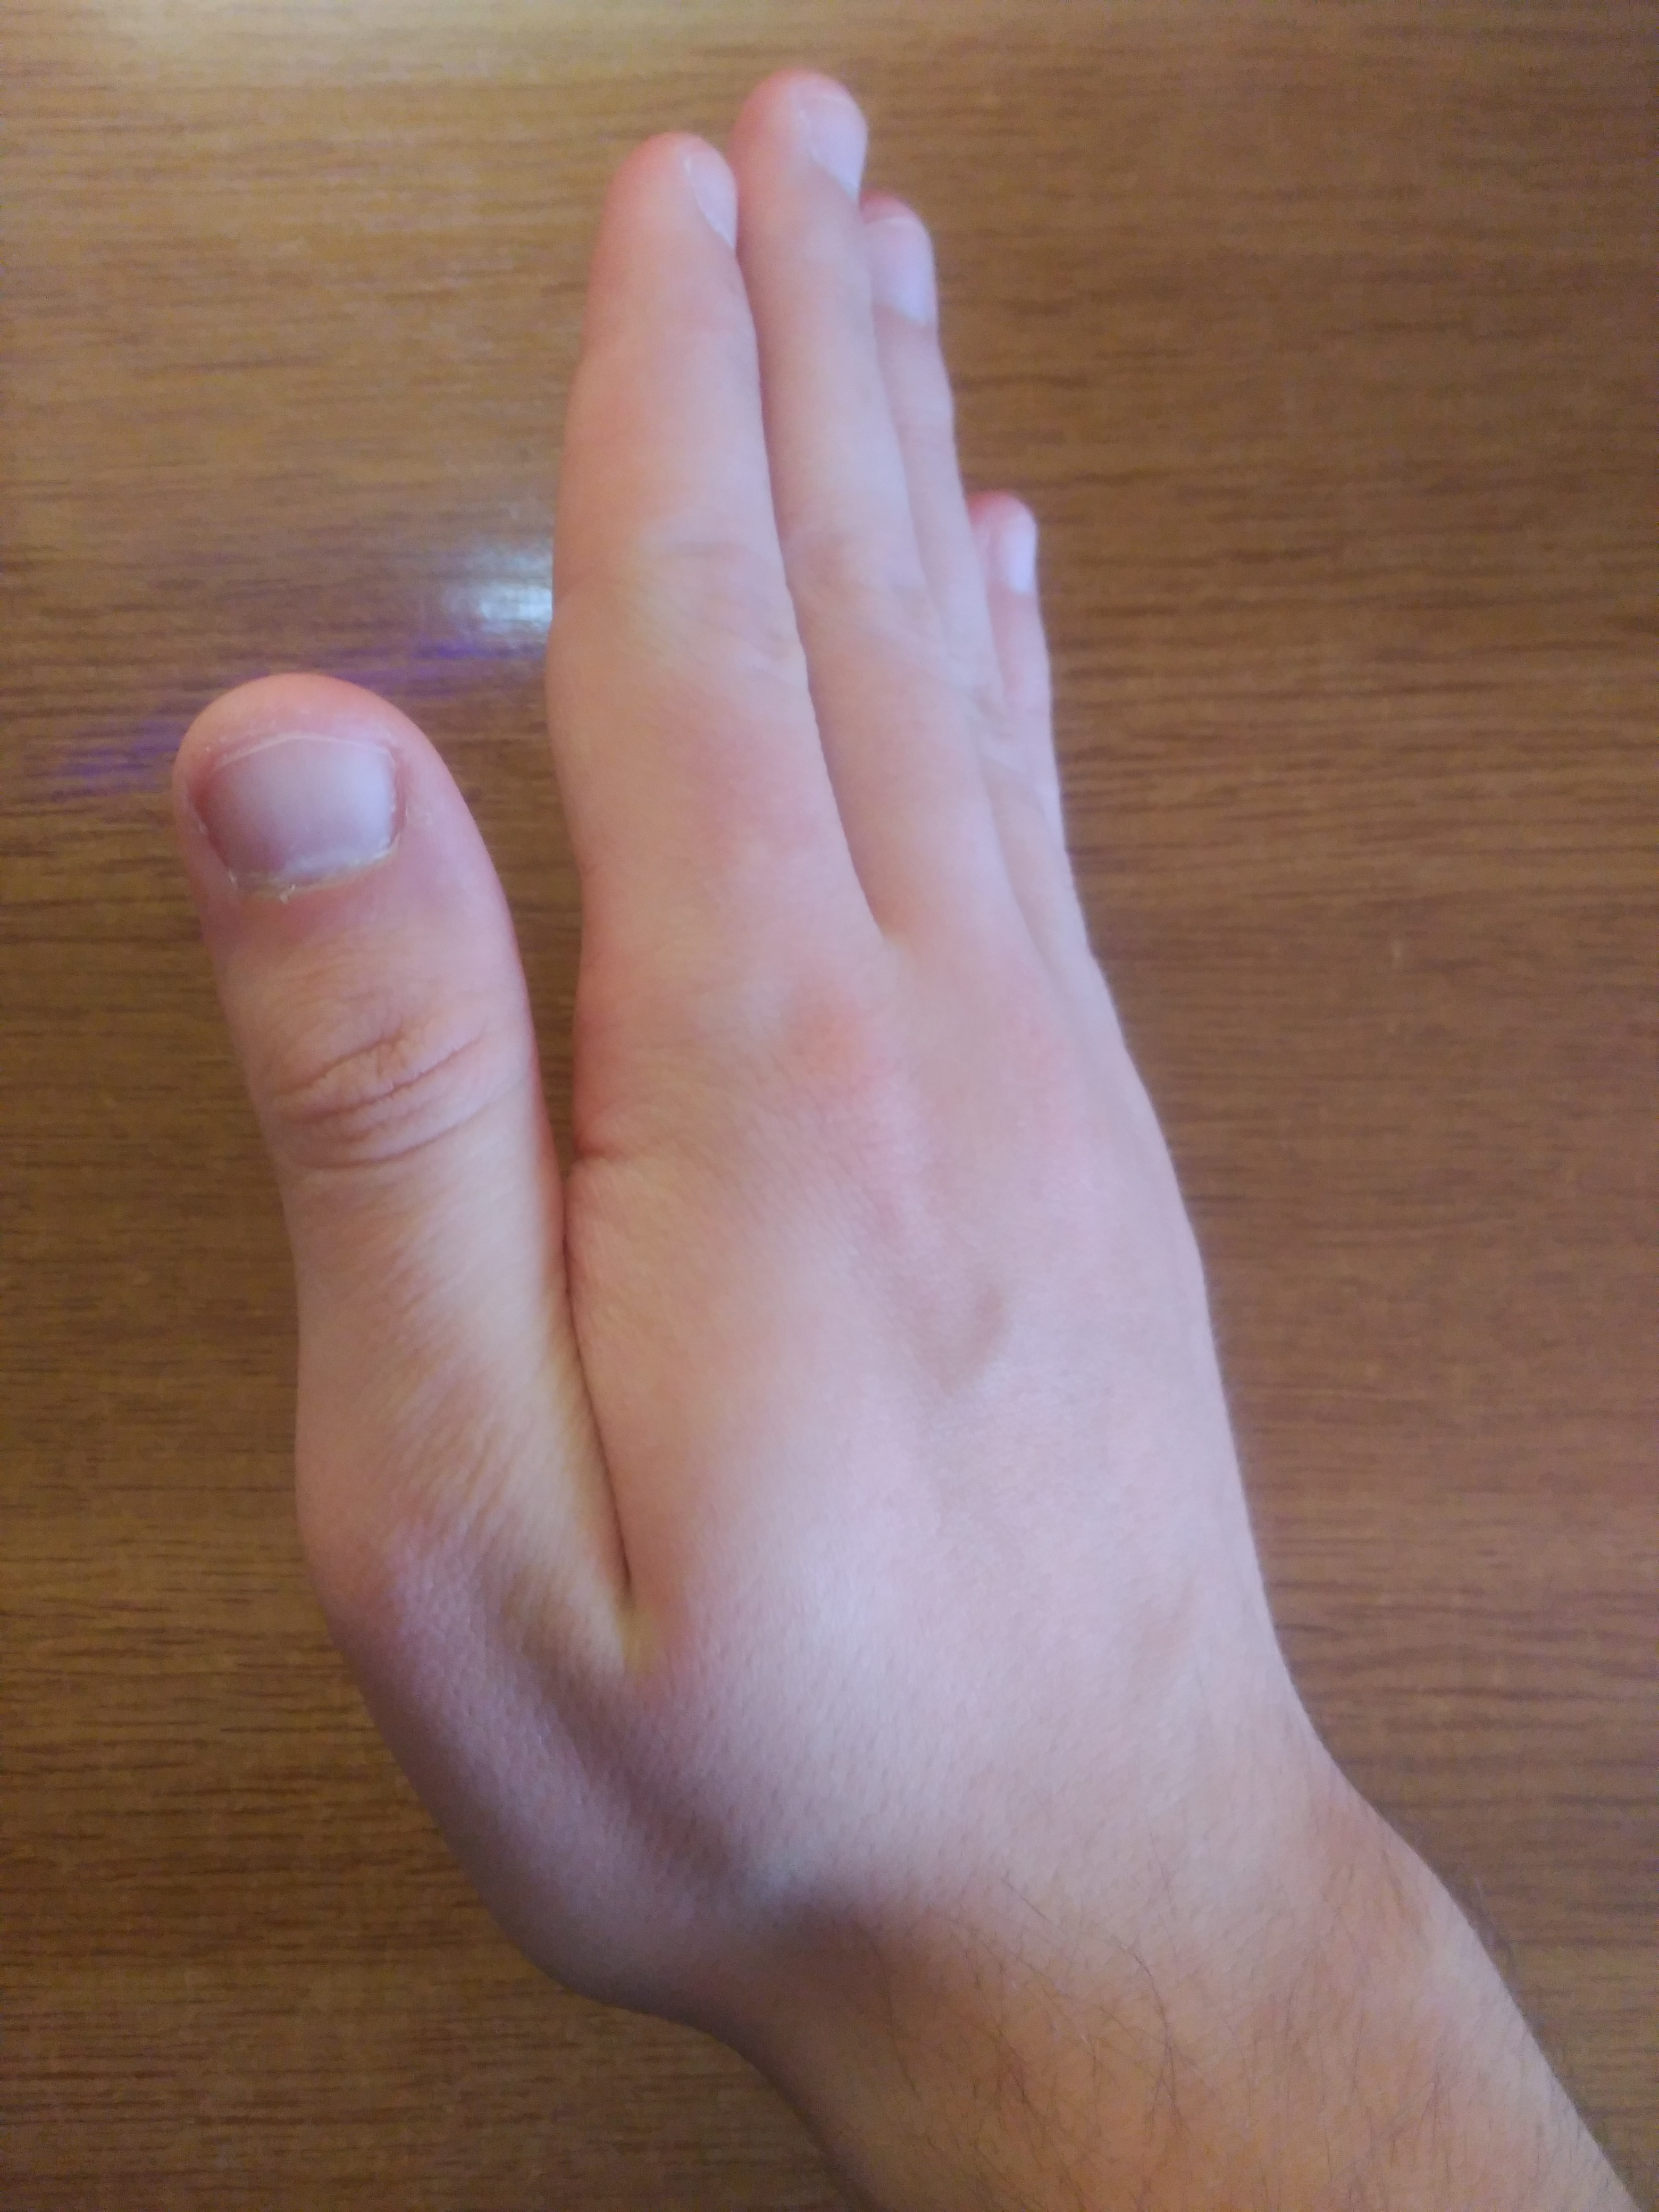
\includegraphics[scale=0.044]{./Imagenes/rota_antihorario.jpg}
		\caption{Mano hacia a la derecha}
	\end{subfigure}
	\caption{Gesto para rotar la figura entorno al eje Y}
	\label{gesto2}
\end{figure}

Como podemos observar en este caso tenemos que comprobar la orientación de la palma de la mano para controlar este movimiento. Para poder hacer esto primero tomamos el vector normal de la palma mediante el atributo `\textbf{hand.PalmNormal}' y lo convertimos a un vector tridimensional. El umbral que hemos detectado que funciona mejor para este gesto es aquel que tiene la componente X del vector normal con valores en el intervalo $(-0.3 \ , \ 0.6)$.

\vspace{10px}

Si el vector normal de la palma apunta hacia la derecha entonces giramos en sentido horario, esto sería inclinar la mano a la izquierda. De forma análoga si el vector normal apunta hacia la izquierda es porque estamos inclinando la mano a la derecha y por tanto giramos en sentido antihorario. La rotación se hace a velocidad constante y al igual que en el gesto anterior sólo lo hacemos cuando la mano detectada es la mano derecha, por lo que controlamos dicho evento.

\subsection{Rotación con respecto al eje X}

Para proseguir hemos implementado también una rotación entorno al eje X para poder visualizar la estatua por arriba y por abajo. Tenemos que tener en cuenta que esta rotación no es completa, es decir, no giramos la estatua 360 grados entorno al eje X ya que hemos considerado que lo más práctico es poder obtener una vista cenital y el resto de los ángulos se pueden apreciar rotando la figura con el gesto anterior. Este gesto se realiza inclinando la mano hacia abajo o arriba tal y como se muestra en la siguiente imagen:

\begin{figure}[!h]
	\centering
	\begin{subfigure}{0.32\textwidth}
		\centering
		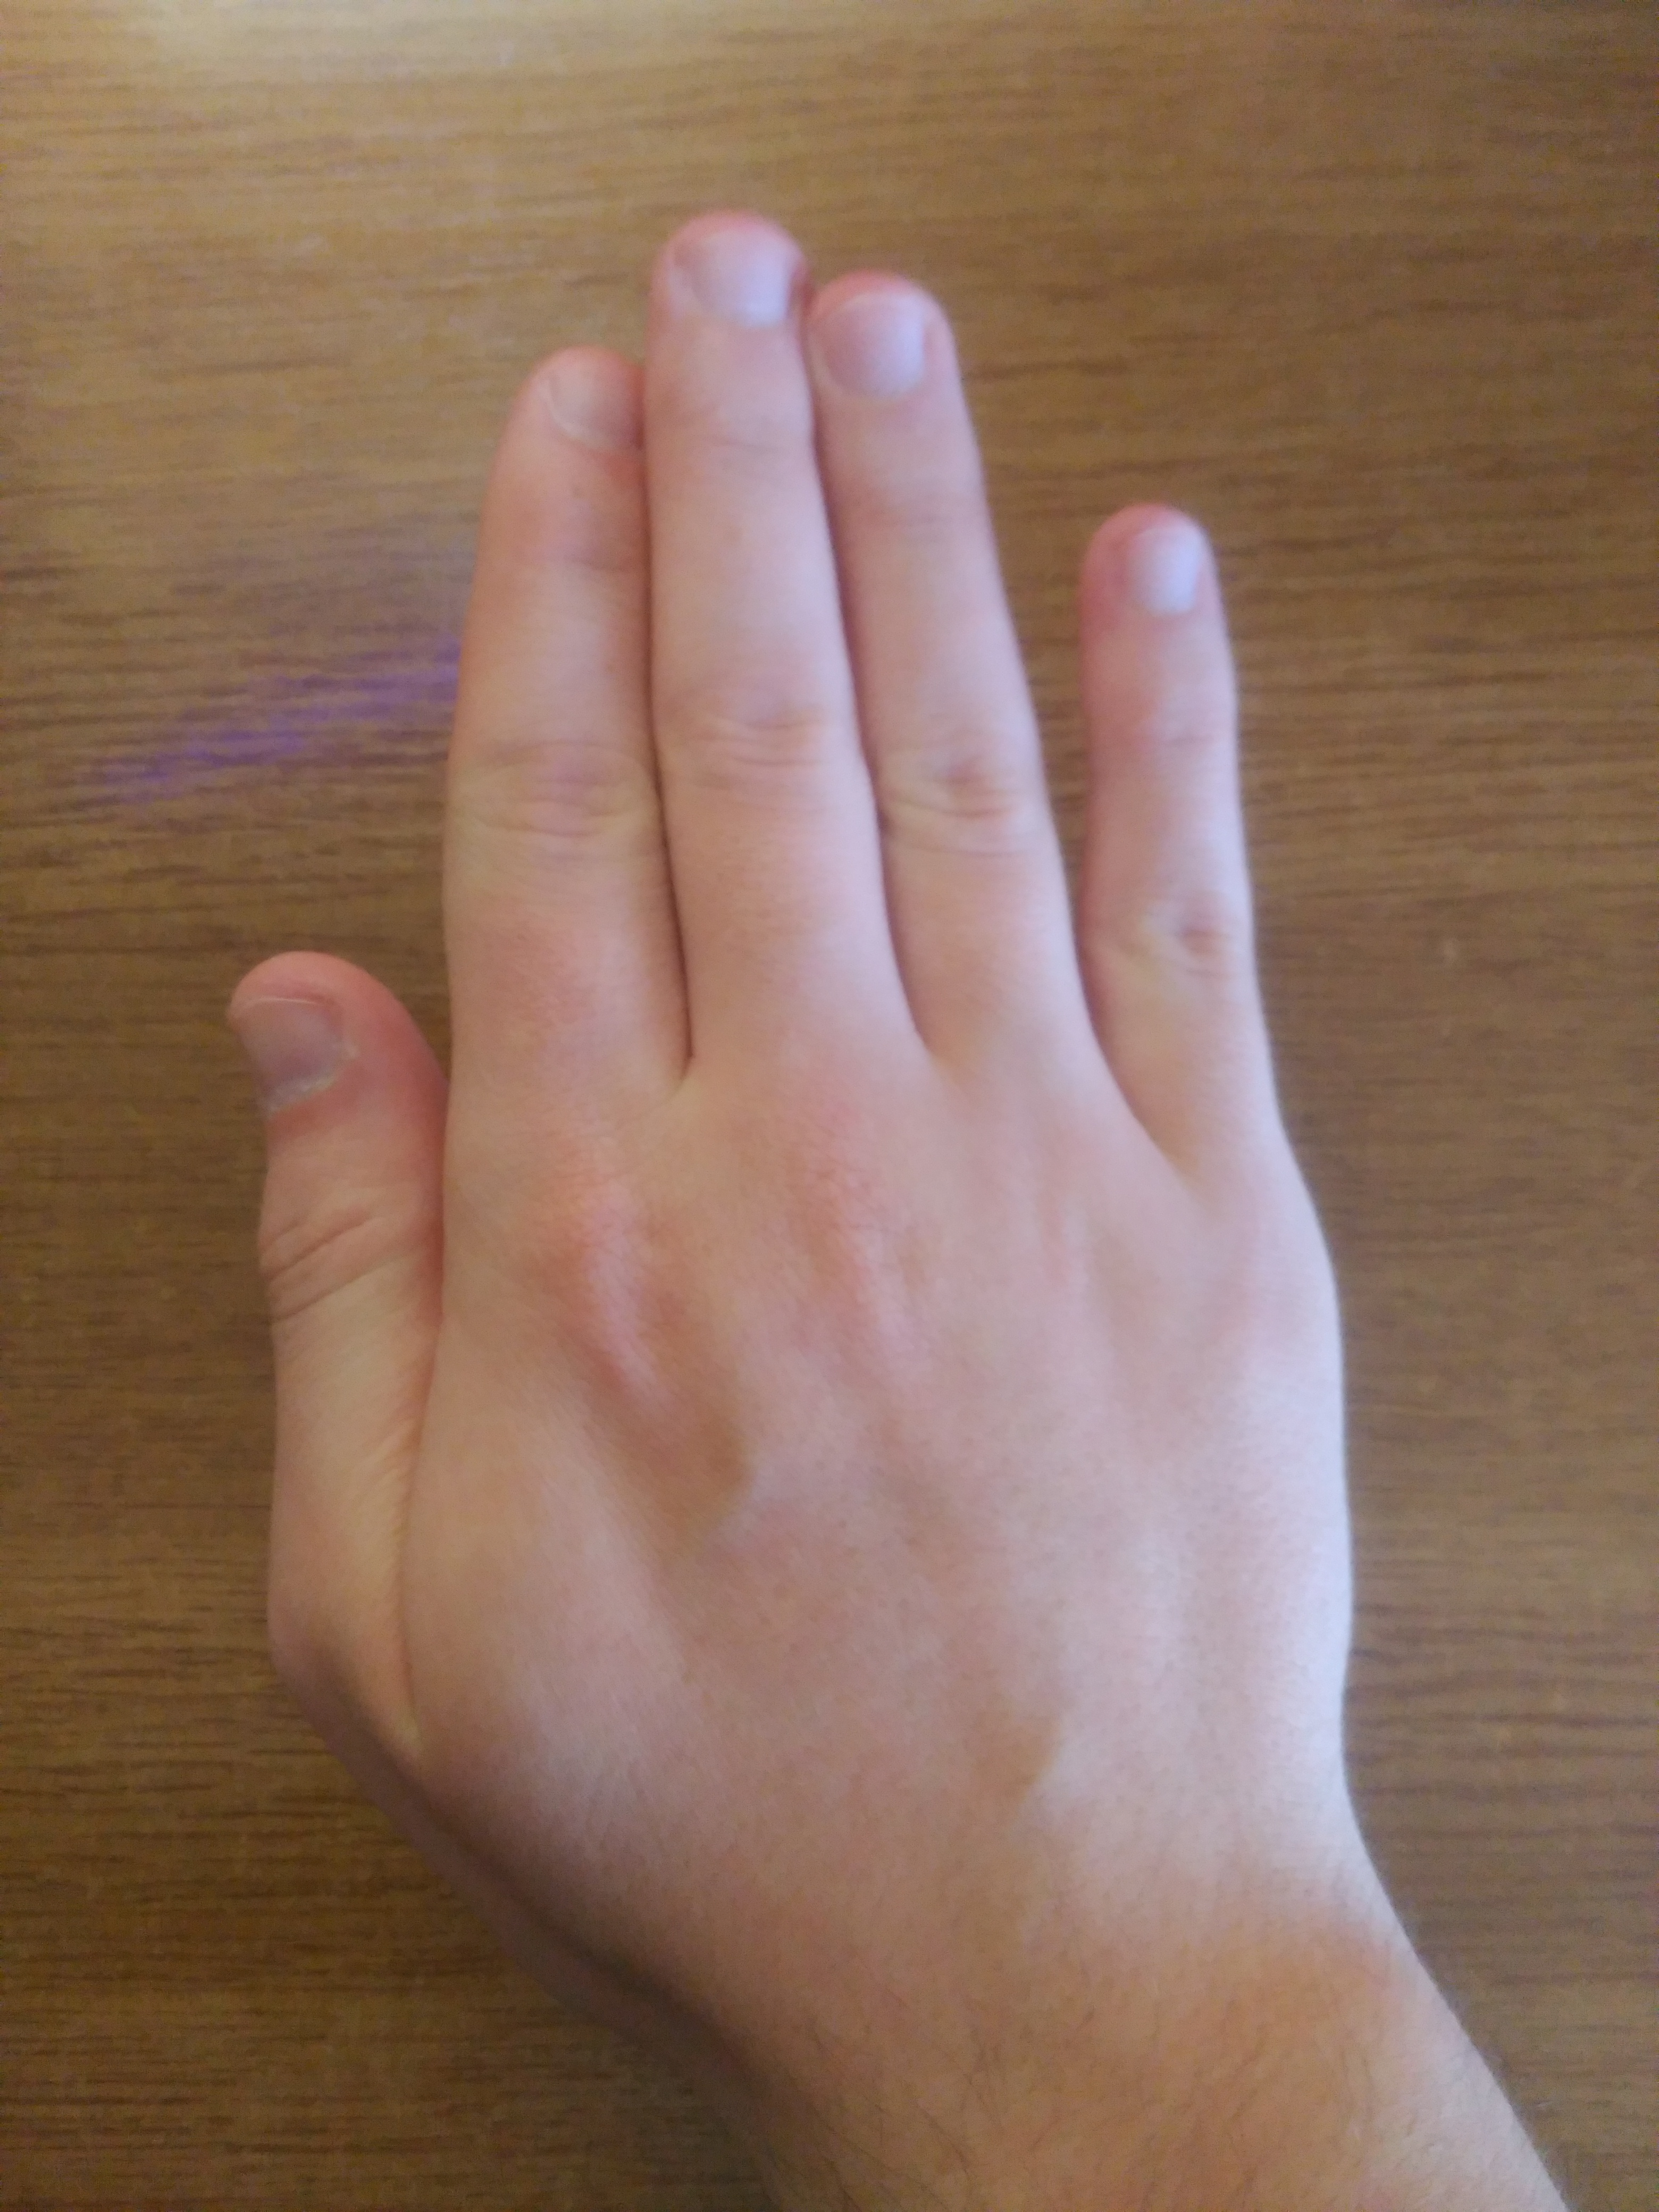
\includegraphics[scale=0.044]{./Imagenes/normal.jpg}
		\caption{Mano sin inclinar}
	\end{subfigure}
	\begin{subfigure}{0.33\textwidth}
		\centering
		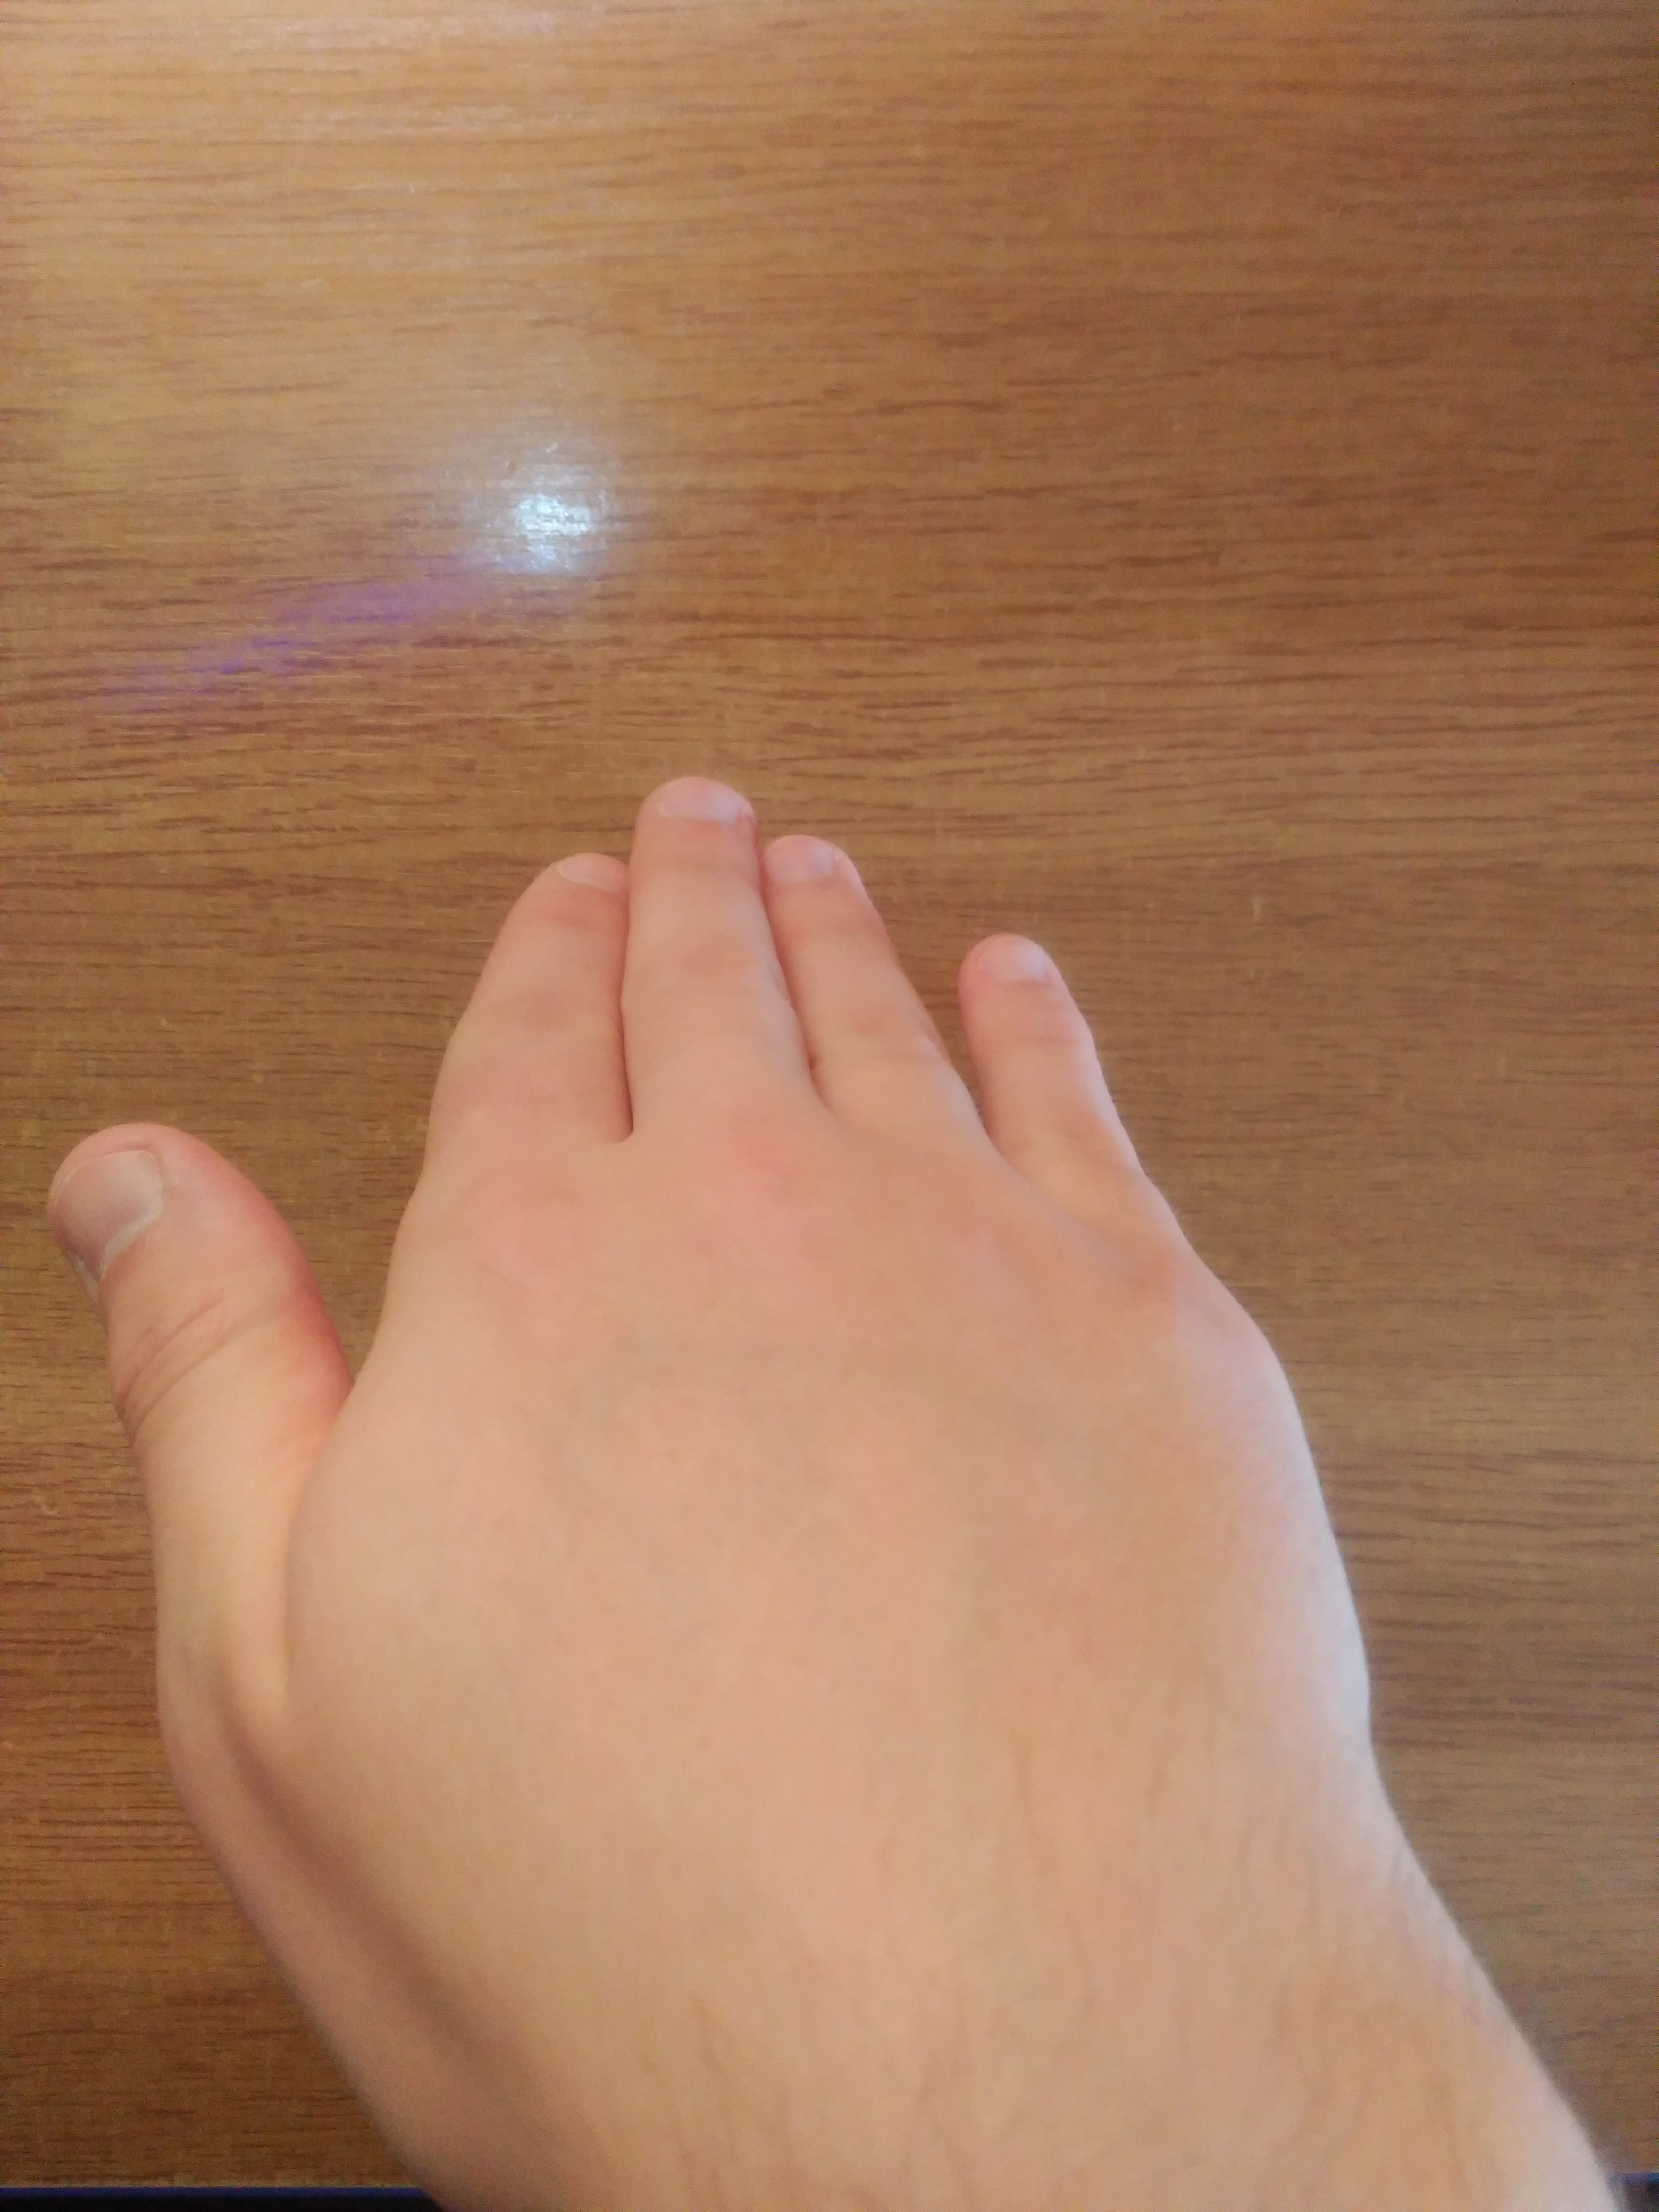
\includegraphics[scale=0.044]{./Imagenes/vista_desde_arriba.jpg}
		\caption{Mano hacia abajo}
	\end{subfigure}
	\begin{subfigure}{0.33\textwidth}
		\centering
		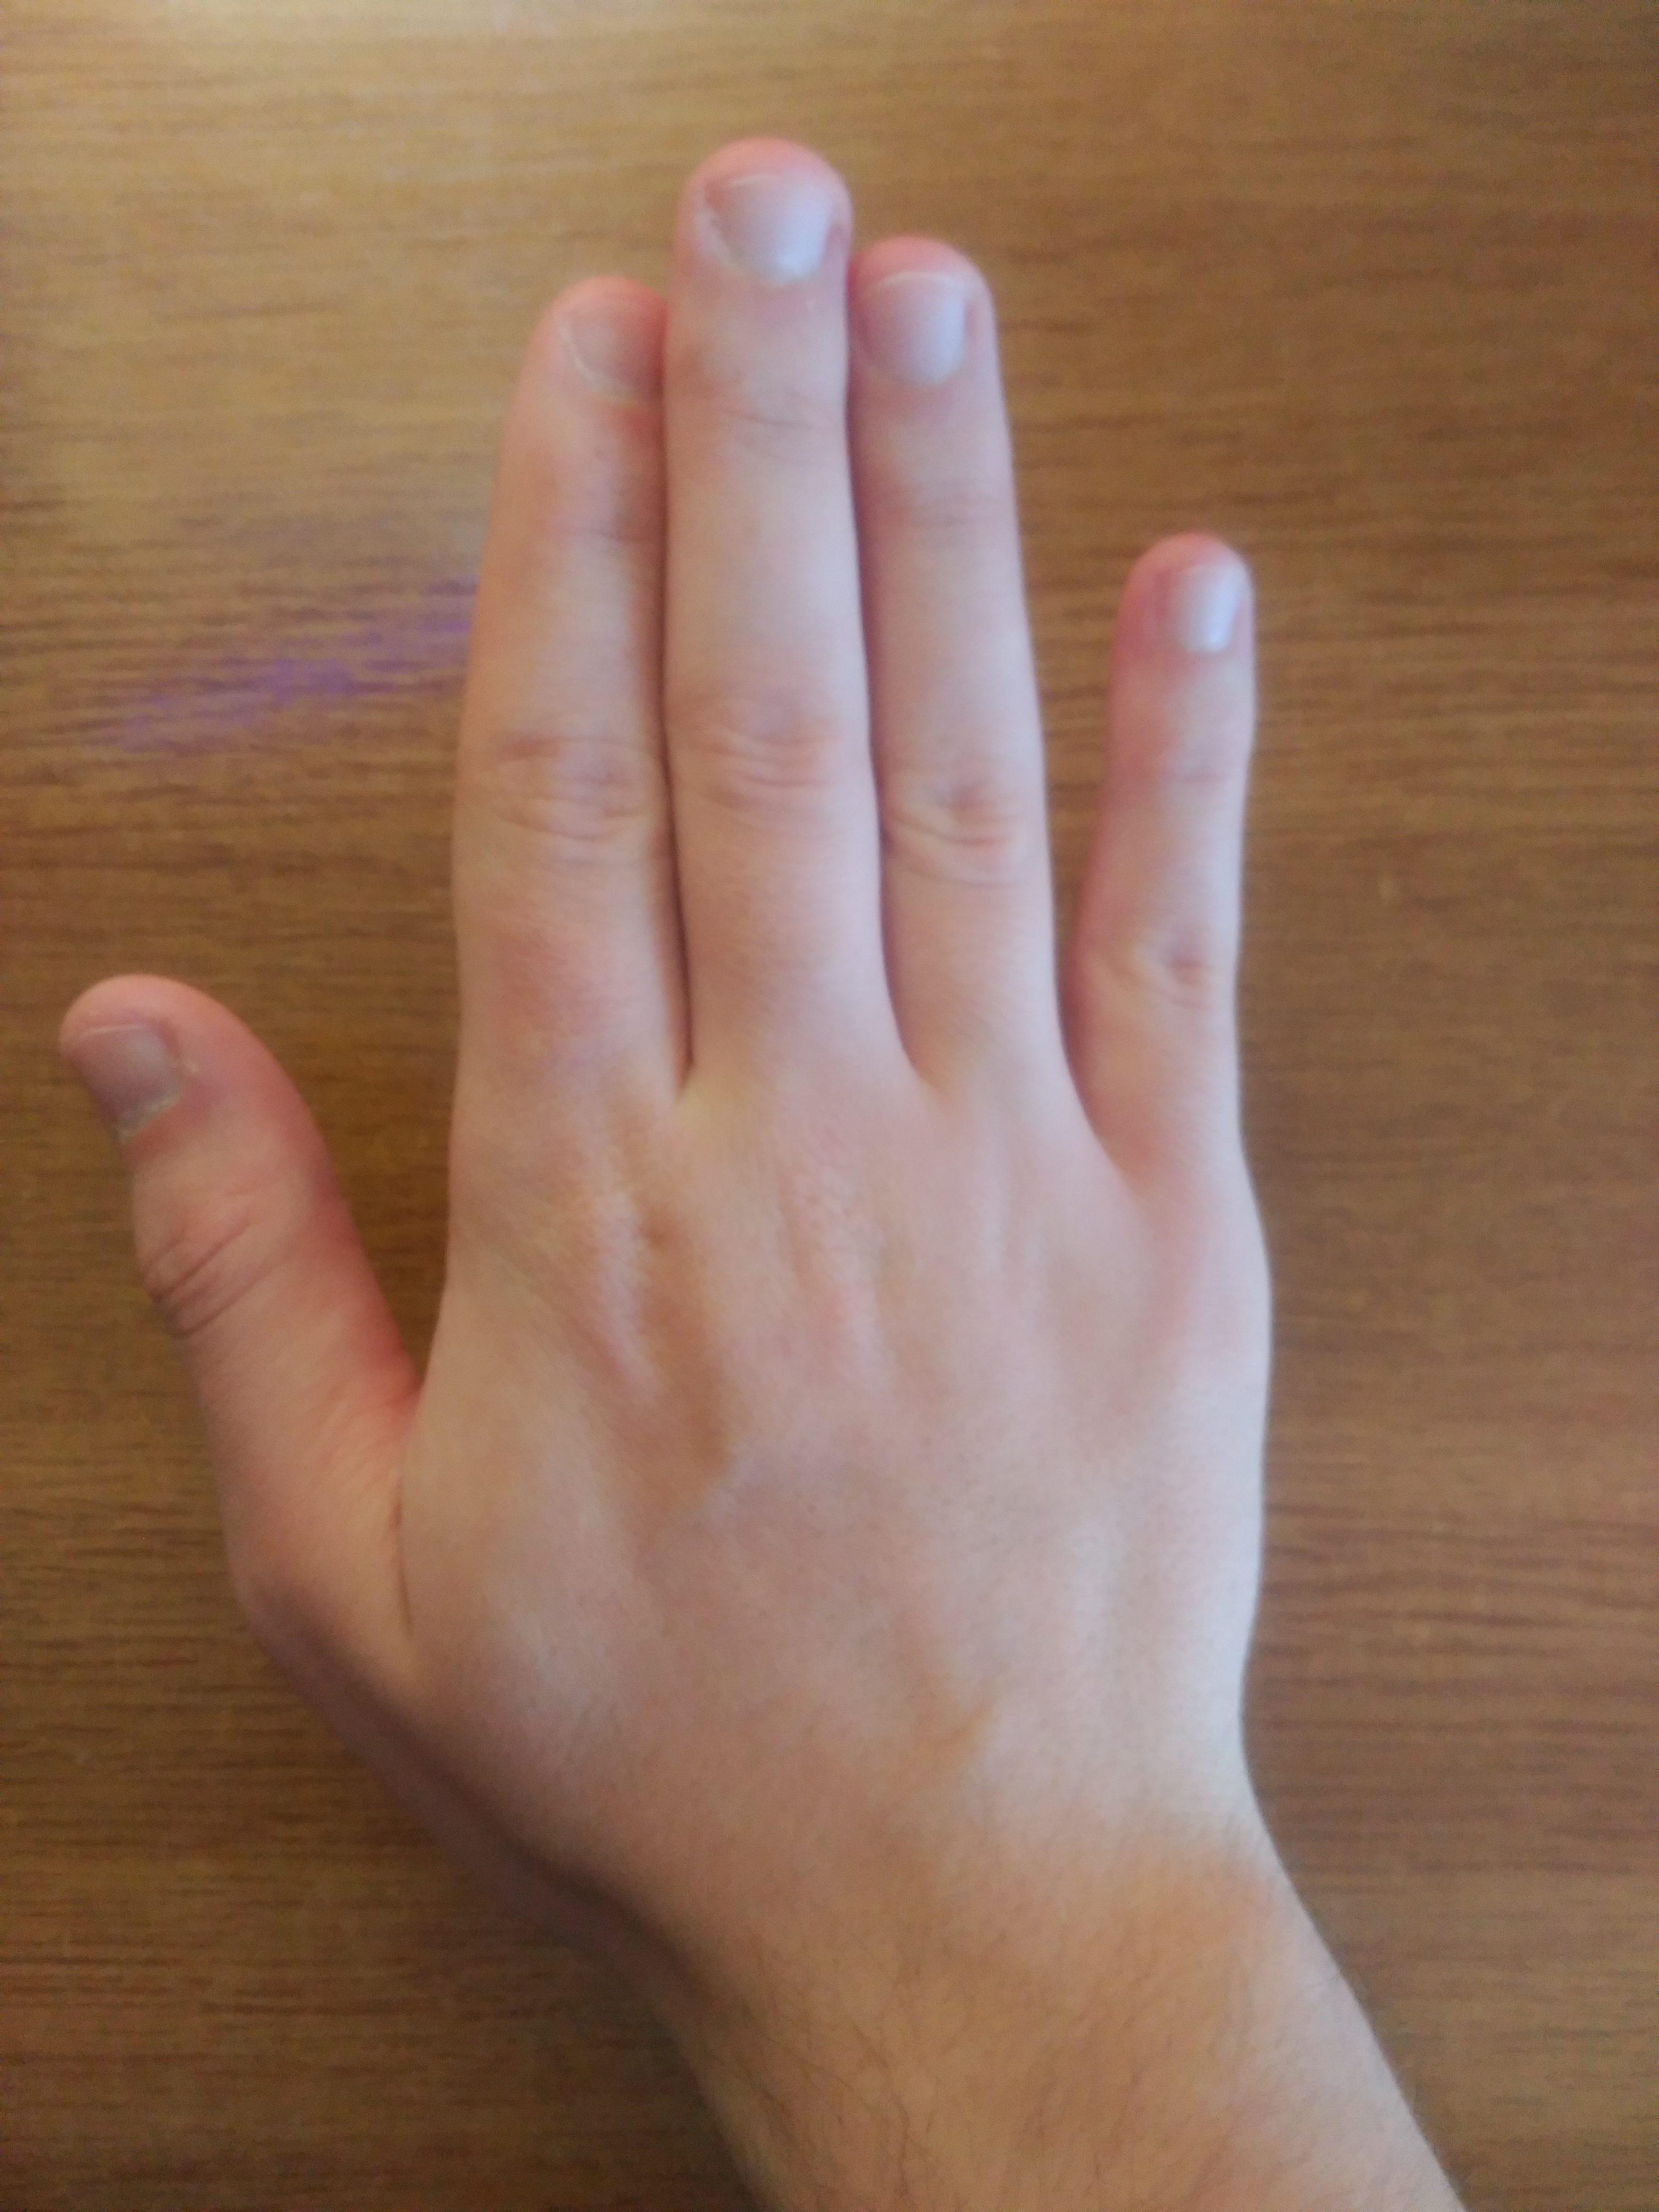
\includegraphics[scale=0.044]{./Imagenes/vista_desde_abajo.jpg}
		\caption{Mano hacia arriba}
	\end{subfigure}
	\caption{Gesto para rotar la figura entorno al eje Y}
	\label{gesto3}
\end{figure}

La implementación de este gesto recae, al igual que en el anterior, en el control del vector normal de la palma. Si antes comprobábamos que la componente X del vector normal estuviera en un rango concreto ahora es la componente Y la que nos interesa. El valor de esta componente del vector normal tiene que estar en el intervalo $(-0.3 \ , \ 0.3)$ ya que es el que hemos comprobado que mejor nos funciona. Una vez comprobado esto la estatua se rota entorno al eje X de forma proporcional a la componente X del vector normal. Lo que obtenemos con esto es que la figura no rote indefinidamente, si no que rote únicamente hasta que obtengamos la vista superior e inferior de la misma previniendo un giro libre del modelo. 

\subsection{Zoom}

Es conveniente para este tipo de aplicaciones tener también una opción de zoom para poder ampliar y ver mejor los detalles. Además cabe recordar que nuestra aplicación no sólo está pensada para modelos como estatuas, si no también para edificios en los que será conveniente tener la opción de poder visualizarlo por dentro gracias al zoom. Este gesto se realiza igual que cuando simulamos tener una cámara en nuestras manos, veamoslo en la siguiente imagen:

\begin{figure}[!h]
	\centering
	\begin{subfigure}{0.48\textwidth}
		\centering
		\includegraphics[scale=0.2]{./Imagenes/zoom1.jpg}
	\end{subfigure}
	\begin{subfigure}{0.48\textwidth}
		\centering
		\includegraphics[scale=0.2]{./Imagenes/zoom2.jpg}
	\end{subfigure}
	\caption{Gesto para aplicar zoom a la figura}
	\label{gesto4}
\end{figure}

La idea de este gesto es que podemos acercarnos la imagen si alejamos los dedos entre sí o alejarnos de la misma si los acercamos.

\vspace{10px}

Para la implementación de este gesto tenemos que hacer varias comprobaciones. Para empezar en este caso necesitamos tener dos manos en escena, de forma que tenemos que comprobar que el vector de manos tenga dos elementos. Además tenemos que comprobar que el dedo corazón, anular y meñique están contraídos en ambas manos y el índice y pulgar están extendidos (hemos comprobado que el comportamiento del dedo pulgar es un tanto irregular cuando es detectado por el Leap Motion por lo que esta condición teórica se traduce en la implementación a que únicamente el índice esté extendido). Además debemos controlar la distancia entre los dedos índices de ambas manos para comprobar si entre la iteración anterior y la actual se han alejado o acercado los mismos. Si los dedos se están acercando entonces la estatua se alejará de forma proporcional a la velocidad de ambas palmas y si lo dedos se están acercando la figura se acercará de forma análoga.

\end{document}
